\documentclass{beamer}
\usetheme{afm}

\title{Change of Measure and Its Applications}
\subtitle{Introduction to Libor Market Models}
\course{Advanced Financial Modeling}
\author{\href{mailto:matteo.sani@unisi.it}{Matteo Sani}}

\begin{document}
	\begin{frame}[plain]
		\maketitle
	\end{frame}

\section{Change of Measure}
\begin{frame}{Few Definitions}

%equivalent measure
%martingale measure

It may be helpful to explain (and recall) some of the more technical terms we are going to use.\newline

\textbf{Sample space}: all possible future states or outcomes ($\Omega$) of a random process.\newline

\textbf{(Probability) Measure} ($\mathcal{P}, \mathcal{Q}\ldots$): is a mapping which associates a probability to each element in the sample space. Two measures are \textbf{equivalent} if they agree "on what is possible". Note the word \emph{possible}: the two measures can have different probabilities for the same event, but must have the same \emph{null-set} $\{x\in {\mathcal {P}}\mid p (x)=0\}$. 
\end{frame}

\begin{frame}{Few Definitions}
\textbf{Contingent claim}: is a derivative whose future payoff depends on the value of another “underlying” asset, or more generally, that is dependent on the realization of some uncertain future event $(S, X\ldots)$.\newline

\textbf{Filtrations}: are totally ordered collections of subsets that are used to model the information that is available at a given point in time ($\mathcal{F}_t$). \newline

\textbf{Martingale}: is a stochastic process for which, at a particular time, the conditional expectation of the next value in the sequence is equal to the present value, regardless of all prior values. It can be imagined as a drift-less process.
\end{frame}

\begin{frame}{Real World Measure $\mathcal{P}$}
\begin{itemize}
	\item When we model derivative prices, we take as given some "true" probability measure $\mathcal{P}$, which assigns probabilities to different states of the world. 
	\item These states in turn affect the path of security prices. 
	\item And these states plus the corresponding probabilities are supposed to reflect the subjective beliefs of traders or investors about what will happen in the future.
	\item Unfortunately, under $\mathcal{P}$ it is usually quite complicated to price derivatives.
	\item This makes it hard to work out the price process and it is necessary to use simulations techniques.
	% as expected discounted cash-flows, i.e. the discounted price process of a derivative is not a martingale: that is, if $C_t$ is the price of a derivative at time $t$ and $r$ is the short rate (let's take it to be constant for simplicity), it's NOT generally the case that
	%\begin{equation*}
	%	C_t=\mathbb{E}_t^{\mathcal{P}}[e^{-r(s-t)}C_s]
	%\end{equation*}
	\end{itemize}
\end{frame}

\begin{frame}{Changing Measure}
\begin{itemize}
	\item It makes sense to look for a new probability measure which could simplify the pricing process given the correct result at the same time.
	%\item This makes it hard to work out the price process and it is necessary to use simulations techniques. 
	%(Actually, no-arbitrage constructions or the Feynman-Kac formula will give you an explicit PDE whose solution is $C_t$, which will not generally be analytical solvable.)
	\item That's why \textcolor{red}{changes of probability measure are important in mathematical finance} because allow to express derivative prices in closed-form.
	\item At the beginning of the course we have seen how simply by assuming the absence of arbitrage it is possible to define a \textcolor{red}{new measure} under which the price of a derivative is given by the discounted expectation of its payoff.
	\item This result has been formalized by \emph{Harrison} and \emph{Pliska} in 1981. 
	\end{itemize}
\end{frame}

\begin{frame}{Equivalent Martingale Measure}
	\begin{block}{Definition}
	An \textcolor{red}{equivalent martingale measure} $\mathcal{Q}$ is a probability measure on the space $\Omega$ such that
	\begin{enumerate}
		\item $\mathcal{Q}$ is equivalent to $\mathcal{P}$;
		%\item the \textcolor{red}{Radon-Nikodym} derivative is square integrable;
		\item the "discounted asset price" is a $\mathcal{Q}$-martingale
		\begin{equation}
			\mathbb{E}^\mathcal{Q}[D(0,t)S_t|\mathcal{F}_u] = D(0,u)S_u, \quad\text{with }(t>u)
		\end{equation}
	\end{enumerate}
	\end{block}
Harrison and Pliska proved two more fundamental results:
\begin{itemize}
	\item the $\mathcal{Q}$-expectation of the discounted claim payoff is the \textcolor{red}{unique no-arbitrage price};
	\item finally, a financial market is arbitrage free and complete if and only if there exists a unique equivalent martingale measure.
\end{itemize}
\end{frame}

\subsection{Numeraires}
\begin{frame}{Numeraires}
	\begin{itemize}
		\item So what we want is an "artificial" probability measure $\mathcal{Q}$ (i.e. assigning different probabilities to states of the world) under which the discounted derivative process IS a martingale.
		\item The question that arises is: how can we determine the right measure $\mathcal{Q}$ ?
		\item The answer is through \emph{change of numeraire}.
		\item A \textcolor{red}{numeraire} is any strictly positive stochastic process $N_t$ that is taken as a unit of reference when pricing an asset $S_t$
		\begin{equation*}
			\tilde{S_t}:=\frac{S_t}{N_t}, \quad t \ge 0
		\end{equation*}
		%\item On the other hand, a random numeraire may involve new risks, and can allow for arbitrage opportunities.
	\end{itemize}
\end{frame}

\begin{frame}{Numeraires}
	\begin{itemize}
		\item \emph{Deterministic numeraires} are easy to handle as they imply just an algebraic transformation (i.e. do not involve any risk), e.g.
		\begin{itemize}
			\item the exchange rate of the Italian Lira to the Euro was locked at EUR 1 = ITL 1936.27 on 31 December 1998.
		\end{itemize}
		\item When the numeraire is a stochastic process, and we want to move to it, the pricing of a claim has to be changed in order to take into account the new risks (the intrinsic randomness of the new numeraire).
		\item In particular it has to be determined a new probability measure under which the transformed process $\tilde{S_t}$ will be a martingale (changing the numeraire implies a change of the probability measure).
	\end{itemize}
\end{frame}

\begin{frame}{Numeraire Examples (I)}
	\begin{itemize}
		\item \textbf{Money market account.} Given $r_t$, a possibly random and time dependent risk-free interest rate process, let
		\begin{equation*}
			N_t := \exp\left(\int_0^t r_s ds\right)
		\end{equation*}
		In this case 
		\begin{equation*}
			\tilde{S_t}:=\frac{S_t}{N_t}=e^{-\int_0^t r_s ds}S_t, \quad t \ge 0
		\end{equation*}
		represents the discounted price of the asset at time 0.
		\item \textbf{Currency exchange rate.} In this case $N_t := R_t$ denotes e.g. the EUR/SGD exchange rate. Let
		\begin{equation*}
			\tilde{S_t}:=\frac{S_t}{R_t}, \quad t \ge 0
		\end{equation*}
		denotes the price of a local (SG) asset quoted in units of the foreign currency (EUR) (notice the difference with previous ITL/EUR example above).
	\end{itemize}
\end{frame}

\begin{frame}{Numeraire Examples (II)}
	\begin{itemize}
		\item \textbf{Forward numeraire.} The price $P(t,T)$ of a bond paying $P(T,T)=1$ at maturity $T$. In this case
		\begin{equation*}
			N_t := P(t,T)=\mathbb{E}\left[e^{\int_t^T r_s ds}\right]
		\end{equation*}
		Notice that the process $t\rightarrow e^{\int_0^t r_s ds} P(t,T)=\mathbb{E}\left[e^{\int_0^T r_s ds}\right], \quad 0 \le t \le T$
		is a martingale
		\item \textbf{Annuity numeraire.} Processes of the form
		\begin{equation*}
			N_t = P(t, T_0, T_n) := \sum_{k=1}^{n}(T_k - T_{k-1})P(t, T_k), \quad 0 \le t \le T
		\end{equation*}
		where $P(t,T_1),P(t,T_2),\ldots,P(t,T_n)$ are bond prices with maturities $T_1 < T_2 < \ldots < T_n$.
	\end{itemize}
\end{frame}

%	\begin{block}{Definition}
%	A probability distribution (measure) $\mathcal{Q}^N$ on the sample space $\Omega$ of possible market scenarios is said to be a \textcolor{red}{risk-neutral measure} if, for every asset $A$, and \textcolor{red}{numeraire} $N$, the price of $A$ at time $t=0$ is the \emph{discounted expectation}, under $\mathcal{Q}^N$, of the price at time $t$, that is
%	\begin{equation}
%		\frac{S_0}{N_0} = \mathbb{E}^{\mathcal{Q}^N}\left[\frac{S_t}{N_t}\bigg| \mathcal{F}_t\right]
%		\label{eq:risk_neutral_pricing}
%	\end{equation}
%	The discounted value process is then a martingale.
%	\end{block}
%	\begin{itemize}
%	\item We could in general assign any probabilities we wanted to states of the world, but expectations wrt these measures would generally not correspond to anything in the real world. 
%	\item For the right choice of measure $\mathcal{Q}^N$, expectations wrt $\mathcal{Q}^N$ actually give the (real-world) prices of derivatives.
%	\end{itemize}
%\end{frame}

\subsection{Radon-Nikodym Derivative}
\begin{frame}{Radon-Nikodym Derivative}
\begin{itemize}
	\item It remains to understand how to pass from a numeraire to another, and hence by a measure to another in an arbitrage free setting.
	\item Notice that until now we have implicitly assumed the bank account $B$ as numeraire.
	\end{itemize}
\begin{block}{Definition}
When two measures are equivalent it is possible to express the first in terms of the second through the \textcolor{red}{Radon-Nikodym derivative}. Indeed there exists a martingale process $\zeta_t$ such that
\begin{equation*}
	\mathcal{Q}^* =\int_{A} \zeta_t(\omega)d\mathcal{Q}(\omega)
\end{equation*}
which can be written in a more concise form as
\begin{equation}
	\frac{d\mathcal{Q}^*}{d\mathcal{Q}} = \zeta_t
	\label{eq:radon_nikodym_der}
\end{equation}
\end{block}
\end{frame}

\begin{frame}{Intuition from Expected Value}
	\begin{itemize}
		\item Notice that we can write the expected value of a generic function $\Pi(x)$ under a measure $\mathcal{F}$, with associated density function $f(x)$ as
		\begin{equation*}
			\mathbb{E}^\mathcal{F}=\int\Pi(x)f(x)dx
		\end{equation*}
		\item Suppose there exists a function $g(x)$, which satisfies the mathematical conditions required to be a density function. Then we can write
		\begin{equation*}
			\mathbb{E}^\mathcal{F}=\int\Pi(x)f(x)\frac{g(x)}{g(x)}dx
		\end{equation*}
		\item If we define $\psi(x)=\Pi(x)\frac{f(x)}{g(x)}$ the expected value can be written as 
		\begin{equation*}
			\int\psi(x)g(x)dx=\mathbb{E}^\mathcal{G}\left[\psi(x)\right]=\mathbb{E}^{\mathcal{G}}\left[\Pi(x)\frac{f(x)}{g(x)}\right]=\mathbb{E}^\mathcal{F}\left[\Pi(x)\right]
		\end{equation*}
	\end{itemize}
\end{frame}

\begin{frame}{Radon-Nikodym Derivative}
\begin{itemize}
	\item The expectations corresponding to the two measures are related by
	\begin{equation*}
		\mathbb{E}^*[X] = \mathbb{E}\left[X\frac{d\mathcal{Q}^*}{d\mathcal{Q}}\right]
	\end{equation*}
	\item In case of a conditioned expectation
	\begin{equation}
		\mathbb{E}^*[X|\mathcal{F}_t] = \frac{\mathbb{E}\left[X\cfrac{d\mathcal{Q}^*}{d\mathcal{Q}}\bigg|\mathcal{F}_t\right]}{\mathbb{E}[\rho_t|\mathcal{F}_t]}
		\label{eq:conditioned_expectation}
	\end{equation}
	which is an equivalent formulation of the famous \emph{Bayes theorem}
 	\begin{equation*}
		P(A|B)=\frac{P(B|A)P(A)}{P(B)}
	\end{equation*}
\end{itemize}
\end{frame}

\subsection{Change of Numeraire}
\begin{frame}{Change of Numeraire}
	\begin{block}{Theorem}
	Assume exists a numeraire $N_t$ and a measure $\mathcal{Q}^N$, equivalent to $\mathcal{P}$, such that the price of any traded asset $S_t$ relative to $N$ is a martingale under $\mathcal{Q}^N$
	\begin{equation*}
		\frac{S_t}{N_t} = \mathbb{E}^N\left[\frac{S_T}{N_T}\bigg|\mathcal{F}_t\right],\quad 0\le t \le T
	\end{equation*}
	Let $U$ be another arbitrary numeraire. Then there exists a measure $\mathcal{Q}^U$, also equivalent to $\mathcal{P}$, such that the price of any traded asset $X_t$, normalized to $U$, is a martingale under $\mathcal{Q}^U$
	\begin{equation*}
		\frac{X_t}{U_t} = \mathbb{E}^U\left[\frac{X_T}{U_T}\bigg|\mathcal{F}_t\right],\quad 0\le t \le T
	\end{equation*}
	\end{block}
\end{frame}	

\begin{frame}{Change of Numeraire}
	\begin{block}{Theorem continued}
		The Radon-Nikodym derivative defining the measure $\mathcal{Q}^U$ is given by
		\begin{equation}
			\frac{d\mathcal{Q}^U}{d\mathcal{Q}^N} = \frac{U_T N_0}{U_0 N_T}
			\label{eq:radon_nikodym_der2}
		\end{equation}
	\end{block}	
	Let's prove first this second part.
	By definition of $\mathcal{Q}^N$, for any asset price $Z$ holds
	\begin{equation*}
		\begin{cases}
		\cfrac{Z_0}{N_0} = 
		\mathbb{E}^N\left[\cfrac{Z_T}{N_T}\right] \\
		\cfrac{U_0}{N_0}\mathbb{E}^U\left[\cfrac{Z_T}{U_T}\right] = \cfrac{\cancel{U_0} Z_0}{N_0 \cancel{U_0}} = \cfrac{Z_0}{N_0}
		\end{cases}\implies \mathbb{E}^N\left[\frac{Z_T}{N_T}\right] = \mathbb{E}^U\left[\frac{U_0 Z_T}{N_0 U_T}\right]
	\end{equation*}
	since both equal $Z_0/N_0$. 
\end{frame}
	
\begin{frame}{Change of Numeraire}
	Also, by definition of Radon-Nikodym derivative
	\begin{equation*}
		\mathbb{E}^N\left[\frac{Z_T}{N_T}\right] = \mathbb{E}^U\left[\frac{Z_T}{N_T} \frac{d\mathcal{Q}^N}{d\mathcal{Q}^U}\right]
	\end{equation*}
	But from the previous result
	\begin{equation*}
	\mathbb{E}^N\left[\frac{Z_T}{N_T}\right] = \mathbb{E}^U\left[\frac{U_0 Z_T}{N_0 U_T}\right]
	\end{equation*}
	The arguments of the expectations under $U$ must equal so we get \cref{eq:radon_nikodym_der2}. 
	
	This last equation shows that \textcolor{red}{the risk-neutral price is invariant under change of numeraire.}
\end{frame}

\begin{frame}{Change of Numeraire}
	\begin{itemize}
	\item Now we can prove the first part of the change of numeraire theorem. The conditional expectation formula~\cref{eq:conditioned_expectation} gives
	\begin{equation*}
		\mathbb{E}^U\left[\cfrac{S_T}{U_T}\bigg|\mathcal{F}_t\right]=\cfrac{\mathbb{E}^N\left[\cfrac{d\mathcal{Q}^U}{d\mathcal{Q}^N}\cfrac{S_T}{U_T}\bigg|\mathcal{F}_t\right]}{\mathbb{E}^N\left[\cfrac{d\mathcal{Q}^U}{d\mathcal{Q}^N}\bigg|\mathcal{F}_t\right]}
	\end{equation*}
	\item But 
	\begin{equation*}
		\begin{cases}
		\mathbb{E}^N\left[\cfrac{d\mathcal{Q}^U}{d\mathcal{Q}^N}\cfrac{S_T}{U_T}\bigg|\mathcal{F}_t\right]=\cfrac{N_0 S_t}{U_0 N_t} \\
		\mathbb{E}^N\left[\cfrac{d\mathcal{Q}^U}{d\mathcal{Q}^N}\bigg|\mathcal{F}_t\right]=\cfrac{N_0 U_t}{U_0 N_t}
		\end{cases}\implies
		\frac{S_t}{\cancel{N_t}}=\mathbb{E}^U\left[\cfrac{S_T}{U_T}\bigg|\mathcal{F}_t\right]\frac{U_t}{\cancel{N_t}}
	\end{equation*}
    \end{itemize}
\end{frame}	

\begin{frame}{Change of Numeraire}
	\begin{itemize}
		\item The power of the Theorem we have just proved stems from the fact that we can find a characterization of our process by means of which we can work-out more easily the fundamental pricing formula.
		\item In particular it tells how we can find a measure associated to the new numeraire such that \textcolor{red}{the price of any asset divided by that numeraire is a martingale}.
		\item Also it gives a simple rule to write (the otherwise difficult to derive) Radon-Nikodym derivative.
%		\item For instance, to change from the measure induced by numeraire $B(t)$, the bank account numeraire, to the one induced by the $P(t,T)$, the Radon-Nikodym derivative, $\frac{d\mathcal{Q}^T}{d\mathcal{Q}}$ can be obtained as
%		\begin{equation}
%			\frac{P(t,T) \cdot 1}{B(t)P(0,T)}
%		\end{equation}
	\end{itemize}
\end{frame}

\begin{frame}{Asset Price divided by Numeraire}
Let $B$ be the money bank numeraire and $\mathcal{Q}^B$ the corresponding risk-neutral measure. Also let $N$ be a numeraire (so $N/B$ is a $\mathcal{Q}^B$ martingale). 

Define a new measure by
\begin{equation*}
	\frac{d\mathcal{Q}^N}{d\mathcal{Q}^B} = \frac{N_TB_0}{B_TN_0}
\end{equation*}

Then, for any $P$ such that $P/B$ is a $\mathcal{Q}^B$ martingale
\begin{equation*}
\mathbb{E}^N\left[\frac{P_T}{N_T}\bigg|\mathcal{F}_t\right] = \frac{\mathbb{E}^B\left[\frac{P_T}{N_T}\frac{N_TB_0}{B_TN_0}\bigg|\mathcal{F}_t\right]}{\mathbb{E}^B\left[\frac{N_TB_0}{B_TN_0}\bigg|\mathcal{F}_t\right]}
=\frac{\mathbb{E}^B\left[\frac{P_T}{B_T}\bigg|\mathcal{F}_t\right]}
{\mathbb{E}^B\left[\frac{N_T}{B_T}\bigg|\mathcal{F}_t\right]}
=\frac{P_tB_t}{N_tB_t}=\frac{P_t}{N_t}
\end{equation*}
So $P/N$ is a $\mathcal{Q}^N$ martingale.
\end{frame}

%\begin{frame}{title}
%	VA SPOSTATA DI QUI
%If you assume that you have a Brownian market:
%\begin{equation*}
%\begin{gathered}
%\frac{dN_t}{N_t} = r_tdt + \sigma^N_t dW^B_t \\
%\frac{dP_t}{P_t} = r_tdt + \sigma^P_t dW^B_t \\
%\frac{d\mathcal{Q}^N}{d\mathcal{Q}^B} = \frac{N_TB_0}{B_TN_0} = 
%\exp\left(\int_0^T\sigma_t^N dW^B_t - \frac{1}{2}\int_0^T(\sigma^N_t)^2 dt\right)
%\end{gathered}
%\end{equation*}
%
%By Girsanov, under $\mathcal{Q}^N$,
%\begin{equation*}
%dW^N_t = dW_t^B - \sigma_t^N dt
%\end{equation*}
%is a Brownian motion and using Ito's lemma you can check that
%\begin{equation}
%\frac{d(P_t/N_t)}{P_t/N_t)} = (\sigma^P_t \sigma^N_t)dW^N_t
%\end{equation}
%which also shows that it is a Brownian martingale under $\mathcal{Q}^N$.
%\end{frame}

\subsection{Applications}
\begin{frame}{Examples}
\footnotesize{\tiny {\tiny }}{
\begin{table}[bt]
	 \renewcommand*{\arraystretch}{1.4}
	\begin{tabular}{|l|l|} \hline
		\begin{tabular}{@{}l@{}}
		Any asset divided by the bank account
		$B_t$\\(recall $dB_t = r_t B_t dt$)
		\boxed{\cfrac{S_t}{B_t} = e^{-\int_0^t r_s ds}S_t}
		\end{tabular}
		& \begin{tabular}{l}
		It is a martingale under the\\
		measure $Q^B$ associated to \\
		the bank account numeraire,\\
  		i.e. the risk neutral measure.
		\end{tabular} \\ \hline
		\begin{tabular}{@{}l@{}}
		The forward rate\\
		\boxed{F(t, T_1, T_2) = \frac{1}{T_2-T_1}\left(\frac{P(t,T_1) - P(t,T_2)}{P(t,T_2)}\right)}\\
		can be interpreted as a portfolio of two ZCBs\\
		divided by another ZCB.		
		\end{tabular}
		& \begin{tabular}{l}
		Under the measure $\mathcal{Q}^2$\\ 
		associated to the numeraire\\ 
		$P(\cdot,T_2)$ it is a martingale.\end{tabular}\\ \hline  
		\begin{tabular}{@{}l@{}}
		The swap rate
		\boxed{S_{\alpha,\beta}(t) = \frac{P(t,T_\alpha)-P(t,T_\beta)}{\sum_{i=\alpha+1}^{\beta}\tau_i P(t,T_i)}}
		\\can be interpreted as a portfolio of two ZCBs\\
		divided by a portfolio of ZCBs.		
		\end{tabular}
		& \begin{tabular}{l}
		It is a martingale under the\\
		measure associated to the\\
		annuity numeraire.
		\end{tabular} \\ \hline
	\end{tabular}
\end{table}}
\end{frame}

\begin{frame}{A Useful Separation}
	\begin{itemize}
	\item Until now we have used $B(t)$, the money market account, as numeraire. But it is natural to look for the most convenient numeraire, which minimizes the mathematical difficulties according to the problem at hand.
	\item Given a contingent claim whose payoff at time $T$ is $\chi$, we have the following formula for its price $\Pi$
	\begin{equation*}
	\Pi_\chi(t,T)=\mathbb{E}^B\left[e^{-\int_t^T r_s ds}\chi\bigg|\mathcal{F}_t \right]=B_t\mathbb{E}^B\left[B^{-1}_T\chi|\mathcal{F}_t\right]
	\end{equation*}
	\item If $\chi$ and the short rate process were independent under $\mathcal{Q}^B$ (recall $\mathbb{E}[XY]=\mathbb{E}[X]\mathbb{E}[Y]$) then we could write
	\begin{equation*}
	\Pi_\chi(t,T)=\mathbb{E}^B\left[e^{-\int_t^T r_s ds}\bigg|\mathcal{F}_t\right]\mathbb{E}^B\left[\chi|\mathcal{F}_t\right] = P(t,T)\mathbb{E}^B\left[\chi|\mathcal{F}_t\right]
	\end{equation*}
	\end{itemize}
\end{frame}

\begin{frame}{A Useful Separation}
	\begin{itemize}
		\item In general the above separation is not possible due to the interaction between the discount factors and the claim payoff. 
		\item In this, like in other concrete situations, a better numeraire is indeed the ZCB with the same maturity $T$ of the derivative to price $(P(T,T)=1)$.
		\item The forward measure $\mathcal{Q}^T$ (also called the $T$-measure) is defined as the martingale measure for the numeraire process $P(\cdot,T)$, the ZCB maturing in T indeed.
		\item It is easy to see that using \cref{eq:radon_nikodym_der2}, in this case the Radon-Nykodim derivative is given by
		\begin{equation}
			\zeta_t = \frac{d\mathcal{Q}^T}{d\mathcal{Q}^B} = \frac{P(t,T)\overbrace{B(0)}^{=1}}{B_t P(0,T)} ,\quad\left(\zeta_T=\frac{\overbrace{P(T,T)}^{=1}B(0)}{B(T)P(0,T)}=\frac{1}{B(T)P(0,T)}\right)
		\label{eq:radon_nikodym_t_forward}
		\end{equation}
	\end{itemize}
\end{frame}

\begin{frame}{A Useful Separation}
	\begin{itemize}
		\item Applying the change of numeraire to the pricing formula, we get
		\begin{equation*}
			\begin{aligned}
			\Pi_\chi(t,T) & = B_t\mathbb{E}^B\left[B^{-1}_T\chi|\mathcal{F}_t\right] \\
			& = B_t\mathbb{E}^B\left[P(0,T)\zeta_T\chi|\mathcal{F}_t\right]\quad\text{(using RN expression above)}\\
			& = B_tP(0,T)\mathbb{E}^B\left[\zeta_T|\mathcal{F}_t\right]\mathbb{E}^T\left[\chi|\mathcal{F}_t\right]\quad\text{(by \cref{eq:conditioned_expectation})}\\
			& = \cancel{B_tP(0,T)}\frac{P(t,T)}{\cancel{B_tP(0,T)}}\mathbb{E}^T\left[\chi|\mathcal{F}_t\right] \\
			& = P(t,T)\mathbb{E}^T\left[\chi|\mathcal{F}_t\right] \\
			\end{aligned}
		\end{equation*}
		which achieves the desired separation (although under a new measure).
		\item Clearly this particular trick is useful when $\chi$ has known dynamics under the forward measure.
	\end{itemize}
\end{frame}

\begin{frame}{Equivalence between $\mathcal{Q}^B$ and $\mathcal{Q}^T$}
By construction of the martingale measure $\mathcal{Q}^B$, the following relationship holds
\begin{equation*}
\begin{gathered}
\frac{P(t,T)}{B_t}=\mathbb{E}^B\left[\frac{P(T,T)}{B_T}\right]\\[0.3cm]
P(t,T)=\mathbb{E}^B\left[\frac{P(T,T)}{B_T}B_t\right] = \mathbb{E}^B\left[\frac{B_t}{B_T}\right]
\end{gathered}
\end{equation*}
Plugging the result into the Radon-Nikodym derivative gives
\begin{equation*}
	\frac{d\mathcal{Q}^T}{d\mathcal{Q}^B} = \frac{B_t}{B_T}\frac{1}{P(t,T)} =\frac{B_t/B_T}{\mathbb{E}^B[B_t/B_T]}
\end{equation*}	
If interest rates are deterministic then the Radon-Nikodym derivative is 1, hence the two measures are the same.
\end{frame}

\begin{frame}{Clarification on Time}
	\begin{itemize}
		\item Clearly as the Radon-Nikodym derivative is a martingale for valuation time $t$, we have
		\begin{equation}
			\frac{d\mathcal{Q}^U}{d\mathcal{Q}^N}=\frac{U_tN_0}{U_0N_t}
		\end{equation}
		\item So do not confuse the maturity of the numeraire bond $T$ with the times at which you have to take the values of the numeraire, in this case $t$ and 0.
		\item If you want to switch from the $T$ measure to the $S$ measure, i.e. the one induced by the bond $P(.,S)$, for the valuation time $t$ we get
		\begin{equation}
			\frac{d\mathcal{Q}^S}{d\mathcal{Q}^T}=\frac{P(t,S)P(0,T)}{P(t,T)P(0,S)}
		\end{equation}
	\end{itemize}
\end{frame}

\begin{frame}{The Forward Rate Under $\mathcal{Q}^T$}
	\begin{block}{Theorem}
		Consider the forward numeraire $P(t,T)$ and denote with $\mathcal{Q}^T$ its associated measure.
		The forward rate spanning the interval $[S,T]$ is the $\mathcal{Q}^T$ expectation of the future spot rate at time $S$ for the maturity $T$
		\begin{equation}
			\mathbb{E}^T[L(S,T)|\mathcal{F}_t] = F(t;S,T)
		\end{equation}
	\end{block}
\end{frame}

\begin{frame}{The Forward Rate Under $\mathcal{Q}^T$}
	\begin{itemize}
	\item \textbf{Proof:}
		\begin{equation*}
			\begin{gathered}
				F(t;S,T) = \frac{1}{\tau}\left[\frac{P(t,S)-P(t,T)}{P(t,T)}\right] \\[0.3cm]
				F(t;S,T)P(t,T) = \frac{P(t,S)-P(t,T)}{\tau}
			\end{gathered}
		\end{equation*}
	\item This is the price at time $t$ of an asset (difference of two bonds). Therefore by the change of numeraire theorem and by definition of forward measure
		\begin{equation*}
			\frac{F(t;S,T)P(t,T)}{P(t,T)} = F(t,S,T)
		\end{equation*}
		is a \textcolor{red}{martingale} under $\mathcal{Q}^T$ measure. Hence
		\begin{equation*}
			F(t;S,T) = \mathbb{E}^T[F(S;S,T)|\mathcal{F}_t] = \mathbb{E}^T\left[\frac{1}{\tau}\left(\frac{1-P(S,T)}{P(S,T)}\right)\bigg|\mathcal{F}_t\right] = \mathbb{E}^T[L(S,T)|\mathcal{F}_t]
		\end{equation*}
	\end{itemize}
\end{frame}

\begin{frame}{The Forward Rate Under $\mathcal{Q}^T$}
	A similar result can be derived for the corresponding instantaneous quantities
	\begin{equation}
		\mathbb{E}^T[r_t|\mathcal{F}_t] = f(t,T)
	\end{equation}
	Indeed from the definition of $\mathcal{Q}^B$
	\begin{equation*}
		\frac{P(t,T)}{B_t}=\mathbb{E}^B\left[\frac{P(T,T)}{B_T}\bigg|\mathcal{F}_t\right]
	\end{equation*}
	but $P(T,T)=1$ so
	\begin{equation*}
	P(t,T)=\mathbb{E}^B\left[\frac{B_tP(T,T)}{B_T}\bigg|\mathcal{F}_t\right]=\mathbb{E}^B\left[e^{-\int_t^Tr_u du}\big|\mathcal{F}_t\right]
	\end{equation*}
	Differentiating with respect to $T$ ($\frac{d}{dx}\int_c^x f(t)dt=f(x)$)
	\begin{equation*}
	\frac{\partial P(t,T)}{\partial T}=
	\mathbb{E}^B\left[r(T)e^{-\int_t^Tr_u du}\big|\mathcal{F}_t\right]
	\end{equation*}
\end{frame}

\begin{frame}{The Forward Rate Under $\mathcal{Q}^T$}
	Now we can change numeraire to $P(\cdot,T)$ so that, using reciprocal of \cref{eq:radon_nikodym_t_forward} ($\zeta^{-1}=\frac{B_t/B_T}{P(t,T)/P(T,T)}$)
	\begin{equation*}
	\frac{\partial P(t,T)}{\partial T}=
	\mathbb{E}^T\left[r(T)\cancel{e^{-\int_t^Tr_u du}}\frac{P(t,T)}{\cancel{e^{-\int_t^Tr_u du}}}\bigg|\mathcal{F}_t\right]=
	P(t,T)\mathbb{E}^T\left[r(T)|\mathcal{F}_t\right]
	\end{equation*}
	Hence
	\begin{equation*}
	\begin{aligned}
	f(t,T)&=\frac{1}{P(t,T)}\frac{\partial P(t,T)}{\partial T}=
	-\frac{\partial \ln P(t,T)}{\partial T}
	= \mathbb{E}^T\left[r(T)|\mathcal{F}_t\right]=	\mathbb{E}^T\left[f(T,T)|\mathcal{F}_t\right]
	\end{aligned}
	\end{equation*}
	Which demonstrates the initial statement and also shows that \textcolor{red}{the instantaneous forward rate is a martingale under the $T$-forward measure}.
	%
	%\begin{frame}{The Expectation Hypothesis}
	%	\begin{itemize}
		%		\item It is possible to prove the following
		%		\begin{equation}
			%			f(t, T) = \mathbb{E}^{\mathcal{Q}^T}[r(T)|\mathcal{F}_t]
			%		\end{equation}
		%		\item According to the pure expectation hypothesis, the above formula is valid if the expected value is taken under the real probability.
		%		\item Absence of arbitrage makes this incompatible with stochastic interest rates.
		%	\end{itemize}
	%	DA CAPIRE MEGLIO
	%\end{frame}
	%
	
\end{frame}

\subsection{Girsanov Theorem}
\begin{frame}{Girsanov Theorem}
	\begin{itemize}
		\item<1-> We're left with one important question:
		\textcolor{red}{what does the path of an asset price $S_t$ look like under a new measure $\mathcal{Q}$ ?} (we need to know in order to be able to really compute its expectation under $\mathcal{Q}$.)
		\item<2-> \emph{Girsanov's theorem} answers to this question since it tells us, when we change from $\mathcal{P}$ to some other measure $\mathcal{Q}$, how the stochastic part of a process ($W_t$) changes under $\mathcal{Q}$.
		\item<3-> Will see that it evolves as the sum of a Brownian motion under $\mathcal{Q}$ and a drift related to the Radon-Nikodym derivative characterizing $\mathcal{Q}$.
		%\item We therefore want to choose the Radon-Nikodym derivative so that the drift of $W_t$ wrt $\mathcal{Q}$ exactly cancels out the drift of $S_t$, leaving us with a pure diffusion process. 
		\item Under mild technical conditions, the resulting diffusion process will be a martingale, meaning $\mathcal{Q}$ is an \emph{equivalent martingale measure}. ?????????
%		\item It turns out that a price process $C_t$ for a derivative on $S_t$ avoids arbitrage opportunities only if a risk-neutral measure for the price process of the underlying $S$ is also a risk-neutral measure for $C$. 
%		\item So we want to construct a risk-neutral measure for $S$.
%		\item Changing measures change every SDE describing asset prices. The way in which this happens is characterized by the Girsanov theorem.
%		\item Obviously the drift of the SDE of the asset changes. The change of drift is characterized by the Girsanov theorem.
	\end{itemize}
\end{frame}
 
\begin{frame}{Girsanov Theorem}
	\begin{itemize}
		\item So Girsanov's theorem actually solves two problems at once
        \begin{itemize}
    		\item it tells us what new probability measure we want to choose;
    		\item AND that $S_t$ evolves as a pure diffusion process under the new measure. ???????????????????
        \end{itemize}
		\item This allows us to straightforwardly compute the expectation with the risk-neutral pricing formula and explicitly solve for the derivative price.
		%\item The Girsanov theorem shows how a SDE changes due to the changes in the underlying probability measure.
		%Indeed if we change the measure, the drift of the SDE changes while the diffusion coefficient remains the same.
		%It can be useful when it is needed to change the drift coefficient of a SDE.
	\end{itemize}
\end{frame}

\begin{frame}{Girsanov Theorem}
	\begin{block}{Theorem}
	Consider the SDE 
	\begin{equation*}
		dX_t = f_t dt + \sigma_t dW_t
	\end{equation*}
	under $\mathcal{P}$. 
	
	Let be given a new drift $f^*_t$ and assume $\gamma_t=\frac{f_t^*-f_t}{\sigma_t}$ such that $\mathbb{E}\left[\exp\left(\frac{1}{2}\int_0^t\gamma_t^2dt\right)\right]<\infty$.
	Define the measure 
	\begin{equation}
	\frac{d\mathcal{P}^*}{d\mathcal{P}}=\exp\left(-\frac{1}{2}\int_0^t \gamma_s^2 ds + \int_0^t \gamma_s dW_s \right)
	\end{equation}
	Then $\mathcal{P}^*$ is equivalent to $\mathcal{P}$. 
	The Radon-Nikodym derivative process is by construction an \textcolor{red}{exponential martingale}.
	\end{block}
\end{frame}

\begin{frame}{Girsanov Theorem}
	\begin{block}{Theorem continued}
		Also the process
		\begin{equation}
			dW^*_t = -\gamma_s dt + dW_t
		\end{equation} 
		is a Brownian motion under $\mathcal{P}^*$, and 
		\begin{equation*}
			dX_t = f^*_t dt + \sigma_t dW^*_t
		\end{equation*}
	The condition $\mathbb{E}\left[\exp\left(\frac{1}{2}\int_0^t\gamma_t^2dt\right)\right]<\infty$ is a sufficient but non-necessary, and it is know as the \textcolor{red}{Novikov condition}.
	\end{block}
\end{frame}

\begin{frame}{An Example}
\begin{itemize}
	\item Consider the stochastic differential equation
	\begin{equation*}
	dX_t = b(X_t, t) dt + a(X_t, t) dW_t
	\end{equation*}
	\item Let's assume that the drift and diffusion coefficients are such that there exists a unique solution to the equation which is $X$.
	\item We want to find a probability measure $\mathcal{Q}$ such that the drift of $X$ is $\tilde{b}(X_t,t)$ instead of $b(X_t,t)$.
\end{itemize}
\end{frame}

\begin{frame}{An Example}
	\begin{equation*}
	\begin{aligned}
		dX_t &= \tilde{b}(X_t,t) dt+b(X_t,t) dt -\tilde{b}(X_t,t) dt + a(X_t,t) dW_t = \\
        &=\tilde{b_t} dt + (b_t -\tilde{b_t})dt + a(X_t,t) dW_t =\\
		&=\tilde{b_t}dt+ a_t\overbrace{\left(\frac{b_t-\tilde{b_t}}{a_t}\right)}^{\gamma_t}dt + a_t dW_t = \\
        &= \tilde{b_t}dt+a_t dW_t + \gamma_t dt\\
		&=\tilde{b_t}dt+a_t d\tilde{W_t}
		\end{aligned}
		\end{equation*}
		where $d\tilde{W_t}=dW_t+\gamma_t dt$.
\end{frame}

\begin{frame}{An Example}
\begin{itemize}
	\item If the Novikov condition is satisfied then we can apply the Girsanov theorem and we have that
	\begin{equation}
		\mathcal{Q} = \mathbb{E}^\mathcal{P}\left[\exp\left(-\frac{1}{2}\int_0^t \gamma_s^2 ds + \int_0^t \gamma_s dW_s \right)\right]
	\end{equation}
	and that $\tilde{W}$ is a Brownian motion on $\mathcal{Q}$.
	\item In practice, don't need to determine $\mathcal{Q}$. It is enough to know it exists, and the SDE of the process of interest according to the new measure.	
	\end{itemize}
   	\begin{tikzpicture}[remember picture,overlay]
    	\node[xshift=5cm,yshift=-3.9cm] (image) at (current page.center) {
\includegraphics[width=20px]{python_logo}};
    	\node[align = center, yshift=1.45cm, below=of image] {\tiny{\href{shorturl.at/ctCF7}{shorturl.at/ctCF7}}};
    \end{tikzpicture}
\end{frame}


%%* A risk-neutral measure $\mathcal{Q}$ allows us to price things in the following way: 
%%* Suppose that at some time $T$ there is an easy no-arbitrage pricing argument pinning down $C_T$. For instance, if $C$ is the price process of a European call on stock $S$ and $T is the exercise date, then $C_T = (S_T - K)^+$, where $K$ is the strike price. 
%%* In this case, the martingale property wrt $\mathcal{Q}$ implies that
%%
%%𝐶_𝑡=\mathbb{𝐸}^{$\mathcal{Q}$}_𝑡[𝑒^{−𝑟(𝑇−𝑡)}𝐶_𝑇]=\mathbb{𝐸}^{$\mathcal{Q}$}_t[𝑒^{−𝑟(𝑇−𝑡)}(𝑆_𝑇−𝐾)^+]









%* Suppose we model $S$ as 
%
%𝑑𝑆_𝑡=\mu_𝑡 𝑑𝑡 + \sigma_t 𝑑𝑊^{$\mathcal{Q}$}_𝑡
%


%\begin{frame}{title}
%\begin{itemize}
%	\item Let $(\Omega,\mathcal{F}_t, \mathbb{P})$ be a probability space with a standard Brownian motion $W^{\mathbb{P}}$.
%	\item The stochastic process $S_t$ represents the evolution of a risky security price satisfying stochastic differential equation (SDE)
%	\begin{equation*}
%		dS_t = \mu S_t dt + \sigma S_t dW^{\mathbb{P}}_t
%	\end{equation*}
%	\item Let's assume that interest rate $r$ is constant. Therefore
%	\begin{equation*}
%		D(0,t) = e^{-rt}
%	\end{equation*} 	
%	which implies $dD = -re^{-rtdt}$.  
%\end{itemize}
%\end{frame}
%
%\begin{frame}{title}
%	\begin{itemize}
%		\item Define then 
%		\begin{equation*}
%			Y_t = D_t S_t
%		\end{equation*} 
%		that is the present value at time $t$ of the risky security.
%		\item Using Ito's lemma
%		\begin{equation*}
%			\begin{aligned}
%			dY_t &= D_t dS_t + dD_t S_t \\ 
%			&= D_t (\mu S_t dt + \sigma S_t dW^{\mathbb{P}}_t) + S_t (-rD_t dt) \\
%			&= (\mu - r) Y_t dt + \sigma Y_t dW_t^{\mathbb{P}}		
%			\end{aligned}
%		\end{equation*}
%		\item In its integral form it becomes
%		\begin{equation*}
%			Y_t = Y_0 + (\mu - r)\int_0^t Y_s ds + \sigma \int_0^t Y_s dW_s^{\mathbb{P}}
%		\end{equation*}
%	\end{itemize}
%\end{frame}
%
%\begin{frame}{title}
%\begin{enumerate}
%\item Let's set 
%\begin{equation*}
%	
%\end{equation*}
%\end{frame}
%
%
%Radon-Nikodym theorem VIII
%Theorem
%Radon-Nikodym theorem. Given two equivalent probability
%measures P and Q constructed on the measurable space
%(Ω, F), there exists a positive-valued random variable Y such
%that
%Q (A) = E
%P
%[Y IA] .
%Such a random variable Y is often denoted by dQ
%dP
%.
%

%\begin{frame}{Intuition behind the Mathematics}
%	\begin{itemize}
%		\item The following theorem is at the heart of the \emph{no arbitrage} pricing theory.
%		\begin{block}{}
%		The market model does not allow for arbitrage if and only if there exist a martingale measure $\mathcal{Q}^0$ under which the processes
%		\begin{equation}
%		\frac{S_0(t)}{S_0(t)},\frac{S_1(t)}{S_0(t)},\ldots,\frac{S_N(t)}{S_0(t)}
%		\end{equation}
%		behave as martingales under $\mathcal{Q}^0$.
%		\end{block}
%	\end{itemize}
%\end{frame}
%\begin{frame}{Numeraire Pricing}
%	\begin{block}{Theorem (German, El Karoui and Rochet, 1995)}
%		Assume that there exists a numeraire $N$ and a probability measure $\mathcal{Q}^N$ which is equivalent to $\mathcal{P}$ such that, for every traded asset $X$:
%		\begin{equation}
%			\frac{X_t}{N_t} = \mathbb{E}^{\mathcal{Q}^N}\left[\frac{X_T}{N_T}|\mathcal{F}_t\right]
%		\end{equation}
%		Now, given a second arbitrary numeraire $U$, there exists a probability measure $\mathcal{Q}^U$ which is equivalent to $\mathcal{P}$ and such that:
%		\begin{equation}
%			\frac{X_t}{U_t} = \mathbb{E}^{\mathcal{Q}^U}\left[\frac{X_T}{U_T}|\mathcal{F}_t\right]
%		\end{equation}
%	\end{block}
%\end{frame}


%\begin{frame}{Example Approach to Numeraire Change}
%\begin{itemize}
%	\item In lieu of the fundamental theorem we can write
%	\begin{equation}
%	\Pi(0,X)=S_0(0)\mathbb{E}^0\left[\frac{X}{S_0(T)}\right]
%	\end{equation}
%	\item But also
%	\begin{equation}
%	\Pi(0,X)=S_1(0)\mathbb{E}^1\left[\frac{X}{S_1(T)}\right]
%	\end{equation}
%	\item We define the Radon-Nikodym derivative
%	\begin{equation}
%	L_0^1(T)=\frac{dQ^1}{dQ^0}
%	\end{equation}
%\end{itemize}
%\end{frame}
%
%\begin{frame}{Example Approach to Numeraire Change}
%	\begin{itemize}
%		\item Hence we can write ?????????????????
%		\begin{equation}
%			\Pi(0,X)=S_1(0)\mathbb{E}^0\left[\frac{X}{S_1(T)}L_0^1(T)\right]
%		\end{equation}
%		\item After some trivial manipulations
%		\begin{equation}
%			S_0(0)\mathbb{E}^0\left[\frac{X}{S_0(T)}\right]=
%			S_1(0)\mathbb{E}^0\left[\frac{X}{S_1(T)}L_0^1(T)\right]
%		\end{equation}
%		\item Finally
%		\begin{equation}
%			\frac{S_0(0)}{S_0(T)}=\frac{S_1(0)}{S_1(T)}L_0^1(T)		
%		\end{equation}
%	\end{itemize}
%\end{frame}
%
%\begin{frame}{Example Approach to Numeraire Change}
%	\begin{itemize}
%		\item Hence 
%		\begin{equation}
%			L_0^1(T) = \frac{dQ^1}{dQ^0}=			\frac{S_0(0)S_1(0)}{S_1(T)S_0(T)}
%		\end{equation}
%
%	\end{itemize}
%\end{frame}
%
%\begin{frame}{The Theorem}
%\begin{block}{}
%Let $\mathcal{Q}^0$ a martingale measure associated with the numeraire $S_0$ and further suppose that $S_1$ is the positive process of an asset such that
%\begin{equation}
%\frac{S_1(t)}{S_0(t)}
%\end{equation}
%is a martingale under $\mathcal{Q}^0$. Define $\mathcal{Q}^1$ by means of the Radon-Nikodym derivative
%		\begin{equation}
%	L_0^1(t) = \frac{S_0(0)S_1(0)}{S_1(t)S_0(t)}
%\end{equation}
%SBAGLIATI GLI INDICI 0 e t
%Then $\mathcal{Q}^1$ is a martingale measure for $S_1$.
%\end{block}
%\end{frame}

\begin{frame}{Moving Away from $\mathcal{P}$ Measure}
\begin{itemize}
	\item Let's go back to the real-world probabilities.
	\item Assume that a stock price has the following dynamic (Geometric Brownian Motion) under the real-world measure $\mathcal{P}$
	\begin{equation*}
	dS_t = \mu S_t dt + \sigma S_t dW_t
	\end{equation*}
	\item Also the bank account is assumed to be deterministic hence
	\begin{equation*}
	dB_t = rB_tdt\implies B_t = e^{rt}
	\end{equation*}
	\item We want to know what happens to the SDE of the stock with two different numeraires:
	\begin{itemize}
		\item risk-neutral measure (bank account numeraire);
		\item stock measure (stock numeraire).
	\end{itemize}
\end{itemize}
\end{frame}

\begin{frame}{Risk-Neutral Measure Dynamics}
	\begin{itemize}
	\item We have seen that under the bank account induced measure 
	\begin{equation*}
	\cfrac{S_t}{B_t} = \mathbb{E}^B\left[\frac{S_T}{B_T}\bigg|\mathcal{F}_t\right]
	\end{equation*}
	\item So if we define $Z_t=\frac{S_t}{B_t}$, since $Z_t$ is a martingale (no-drift process) it's evolution can be described by
	\begin{equation}
	dZ_t = \sigma Z_t dW_t^B
	\label{eq:z_martingale1}
	\end{equation}
	where $dW_t^B$ is a Brownian motion under the $\mathcal{Q}^B$ measure.
\end{itemize}
\end{frame}

\begin{frame}{Risk-Neutral Measure Dynamics}
\begin{itemize}
	\item By applying Ito's rule to $Z_t$ ???????
	\begin{equation*}
		\begin{aligned}
		d\left(\frac{S_t}{B_t}\right) &= \frac{dS_t}{B_t} + S_t d\left(\frac{1}{B_t}\right) \\ 
		&=\frac{dS_t}{B_t} + S_t d\left(e^{-rt}\right) = \frac{dS_t}{B_t} - S_t re^{-rt}dt \\
		&= \frac{dS_t}{B_t} - r\frac{dS_t}{B_t}dt 
		\end{aligned}
	\end{equation*}
	\item Now substitute for $dS_t$
	\begin{equation*}
		d\left(\frac{S_t}{B_t}\right)= \frac{ \mu S_t dt + \sigma S_t dW_t}{B_t} - r\frac{dS_t}{B_t}dt = \sigma\frac{S_t}{B_t}\left(\frac{\mu - r}{\sigma}dt + dW_t \right)
	\end{equation*}	
\end{itemize}
\end{frame}

\begin{frame}{Risk-Neutral Measure Dynamics}
	\begin{itemize}
	\item In terms of $Z_t$ it becomes
	\begin{equation}
	dZ_t = \sigma Z_t\left(\frac{\mu - r}{\sigma}dt + dW_t \right)
	\label{eq:z_martingale2}
	\end{equation}
	\item Both \cref{eq:z_martingale2} and~\cref{eq:z_martingale1} represent the dynamic of $Z_t$ so they must equal
	\begin{equation*}
		\cancel{\sigma Z_t}dW_t^B = \cancel{\sigma Z_t}\left(\frac{\mu - r}{\sigma}dt + dW_t\right)
	\end{equation*}
	\item Replacing the Brownian Motion into the real-world dynamic
	\begin{equation*}
		\begin{aligned}
		dS_t &= \mu S_t dt + \sigma S_t \left(dW_t^B - \frac{\mu - r}{\sigma}dt\right) \\
		& = \mu S_t dt - \mu S_t dt + rS_t dt + \sigma S_t dW_t^B  = rS_t dt + \sigma S_t dW_t^B
		\end{aligned}
	\end{equation*}
	\item So \textcolor{red}{under the risk-neutral measure the drift equals the risk-free rate}.
\end{itemize}
\end{frame}

\begin{frame}{Stock Numeraire Measure Dynamics}
	\begin{itemize}
	\item Now let's see what happens under the stock numeraire.
	\item Again under the measure $\mathcal{Q}^B$
	\begin{equation*}
	\frac{S_0}{B_0} = \mathbb{E}^B\left[\frac{S_t}{B_t}\bigg|\mathcal{F}_0\right] \implies
	S_0 = \mathbb{E}^B\left[B_0\frac{S_t}{B_t}\bigg|\mathcal{F}_0\right]
	\end{equation*}
	\item Similarly under the measure $\mathcal{Q}^A$ induced by asset numeraire $A$
	\begin{equation*}
	S_0 = \mathbb{E}^A\left[A_0\frac{S_t}{A_t}\bigg|\mathcal{F}_0\right]
	\end{equation*}
	\item Since both expressions represent a price of an asset they must be the same and we can equal the terms inside the expectations.
\end{itemize}
\end{frame}

\begin{frame}{Stock Numeraire Measure Dynamics}
	\begin{equation*}
	\frac{B_0}{B_t}d\mathcal{Q}^B = \frac{A_0}{A_t}d\mathcal{Q}^A\implies \frac{d\mathcal{Q}^A}{d\mathcal{Q}^B}=\frac{B_0A_t}{B_tA_0}
	\end{equation*}
	\begin{itemize}
	\item We know that the solution in the risk-neutral measure of the GBM is (see pg. 14 to 18 of "no\_arbitrage" slides)
	\begin{equation*} 
	A_t = A_0 e^{rt-\frac{1}{2}\sigma^2 t + \sigma W^B_t}
	\end{equation*}
	so we can re-write
	\begin{equation*}
	\frac{d\mathcal{Q}^A}{d\mathcal{Q}^B}=\frac{\cancel{A_0}e^{\cancel{rt}-\frac{1}{2}\sigma^2 t + \sigma W^B_t}}{\cancel{e^{rt}}\cancel{A_0}}=e^{-\frac{1}{2}\sigma^2 t + \sigma W^B_t}
	\end{equation*}
\end{itemize}
\end{frame}

\begin{frame}{Stock Numeraire Measure Dynamics}
\begin{itemize}
	\item From the Girsanov theorem, setting the function $y_t = \sigma$, we get the transformed diffusion process
	\begin{equation*}
	dW_t^A = dW_t^B - \sigma dt 
	\end{equation*}
	\item Substituting back into the risk-neutral dynamics we get
	\begin{equation*}
		\begin{aligned}
			dS_t &= r S_t dt + \sigma S_t dW_t^B = 
			rS_t dt + \sigma S_t (dW_t^A + \sigma dt) \\
			& = (r + \sigma^2)S_t dt + \sigma S_t dW^A_t
		\end{aligned}
	\end{equation*}
\end{itemize}
%\vspace{3cm}
%\footnotesize{Exercise: calculate the drift change for the Vasicek Model in case you change from B(t) to P(0,T) numeraire}
\end{frame}

\begin{frame}{Summarizing the Results}
	\begin{itemize}
	\item To summarize all the results
	\vspace{0.5cm}
	\begin{table}
		\begin{tabular}{llr}
		$(i)$&$dS_t = \textcolor{red}{\mu} S_t dt + \sigma S_t dW_t$ & Real-world measure \\
		$(ii)$&$dS_t = \textcolor{red}{r}S_t dt + \sigma S_t dW_t^B$ & Risk-neutral measure \\
		$(iii)$&$dS_t = \textcolor{red}{(r + \sigma^2)}S_t dt + \sigma S_t dW^A_t$ & Stock measure\\
		\end{tabular}
	\end{table}
	\vspace{0.5cm}
	\item In practical terms, this means that it possible to use equation $(ii)$, instead of equation $(i)$, to simulate future payoffs, and hence that it is possible to get rid of the big problem of the equity premium estimation. Equation $(ii)$ just needs estimates of the risk-free rate $r$ and of the volatility $\sigma$, which can be derived from real market quotes.
	\end{itemize}
	\begin{tikzpicture}[remember picture,overlay]
	\node[xshift=5cm,yshift=-3.7cm] (image) at (current page.center) {
\includegraphics[width=20px]{python_logo}};
	\node[align = center, yshift=1.45cm, below=of image] {\tiny{\href{shorturl.at/rGJQ3}{shorturl.at/rGJQ3}}};
	\end{tikzpicture}
\end{frame}


\begin{frame}{Drift Changes (Generalization)}
	\begin{block}{Proposition}
	Assume that, under the $S$-measure, we have
	\begin{equation*}
	dX_t = \mu^S(X_t)dt + \sigma(X_t)dW^S_t
	\end{equation*}
	where $dW^S_t$ is a $n$-dimensional standard Brownian motion. Under the $U$-measure, we have
	\begin{equation}
	\mu^U_t(X_t) = \mu^S_t(X_t) - \rho\sigma(X_t)\left(\frac{\sigma^S_t}{S_t}-\frac{\sigma^U_t}{U_t}\right)
	\end{equation}
	or
	\begin{equation}
	dW^U_t = dW^S_t + \rho\left(\frac{\sigma^S_t}{S_t}-\frac{\sigma^U_t}{U_t}\right) dt
	\end{equation}
	$\rho$ is the correlation matrix of $<dW^S,dW^U>$ and $\sigma^S_t$ and $\sigma^U_t$ are the (vector) volatilities of numeraires $S$ and $U$. %(one component for each Brownian motion).
	\end{block}
\end{frame}

\begin{frame}{Drift Changes (Proof)}
	We now provide a formal proof of the above proposition in the special case of \textcolor{red}{$n=1$}, in which \textcolor{red}{$\rho=1$}.
	
	Indicate by $\mathcal{Q}^S$ and $\mathcal{Q}^U$ the $S$-measure and $U$-measure. By Girsanov theorem we have the following expression for the Radon-Nikodym derivative
	\begin{equation*}
	\zeta_t = \frac{d\mathcal{Q}^S}{d\mathcal{Q}^U} = e^{-\frac{1}{2}\int_0^t\alpha_s^2 ds + \int_0^t\alpha_s dW_s^U}
	\end{equation*}
	with 
	\begin{equation}
	\alpha_t=\frac{\mu^S_t(X_t)-\mu_t^U(X_t)}{\sigma_t(X_t)}
    \label{eq:alpha_t}
	\end{equation}
	We also know that $\zeta_t$ is an exponential martingale hence its dynamics is such that 
	\begin{equation}
	d\zeta_t=\alpha_t\zeta_tdW_t^U
	\label{eq:dzeta1}
	\end{equation}
\end{frame}

\begin{frame}{Drift Changes (Proof)}
	By the main theorem on numeraire change \cref{eq:radon_nikodym_der2}, and using the fact that $\zeta_t$ is a $\mathcal{Q}^U$ martingale, 
	\begin{equation}
	\zeta_t = \frac{d\mathcal{Q}^S}{d\mathcal{Q}^U} = \frac{U_0S_t}{S_0U_t}
	\label{eq:zeta_numeraire}
	\end{equation}
	thus
	\begin{equation}
	d\zeta_t= \frac{U_0}{S_0}d\left(\frac{S_t}{U_t}\right)= \frac{U_0}{S_0}\sigma_t^{S/U}dW_t^U
	\label{eq:dzeta2}
	\end{equation}
	where $\sigma^{S/U}_t$ is the volatility of the process $S_t/U_t$, which is also a martingale under $\mathcal{Q}^U$. Comparing the two results for $d(S_t/U_t)$ (\cref{eq:dzeta1}, \cref{eq:dzeta2} and using \cref{eq:zeta_numeraire}) we get
	\begin{equation}
		\begin{gathered}
		\alpha_t\zeta_tdW_t^U = \alpha_t\frac{\cancel{U_0}S_t}{\cancel{S_0}U_t}\cancel{dW_t^U}=	\frac{\cancel{U_0}}{\cancel{S_0}}\sigma^{S/U}_t\cancel{dW_t^U} \\
		\alpha_t = \frac{U_t}{S_t}\sigma^{S/U}_t
		\end{gathered}
	\end{equation}
\end{frame}

\begin{frame}{Drift Changes (Proof)}
	Using the definition of $\alpha_t$ (\cref{eq:alpha_t})
	\begin{equation}
	\mu_t^U(X_t)=\mu_t^S(X_t)-\frac{U_t}{S_t}\sigma_t(X_t)\sigma^{S/U}_t
	\label{eq:alpha}
	\end{equation}
	
	Now let $S_t$ and $U_t$ have dynamics under $\mathcal{Q}^U$ given by 
	\begin{equation*}
		\begin{gathered}
			dS_t = (\ldots) dt + \sigma^S dW^U_t\\
			dU_t = (\ldots) dt + \sigma^U dW^U_t 
		\end{gathered}
	\end{equation*}
\end{frame}

\begin{frame}{Intermezzo}
\begin{itemize}
\item One of the classical formulas of differential calculus is Leibniz rule $d(x y) = x(dy) + y(dx)$
\item For stochastic processes this becomes, applying It$\hat{o}$'s formula to the function $F(x^1,x^2) = x^1x^2$
\begin{equation*}
dF(x_i)=\sum_{i=1}^n \frac{\partial F}{\partial x_i}dx_i
+\frac{1}{2}\sum_{i,j=1}^2 \frac{\partial^2 F}{\partial x_i \partial x_j}dx_i dx_j
\end{equation*}
\begin{equation*}
\begin{gathered}
\frac{\partial F}{\partial x}=y,\frac{\partial F}{\partial y}=x \\
\frac{\partial^2 F}{\partial x^2}=0,\frac{\partial^2 F}{\partial x\partial y}=\frac{\partial^2 F}{\partial y\partial x}=1,\frac{\partial^2 F}{\partial y^2}=0\\
\\
d(x^1 x^2) = x^1dx^2 + x^2dx^1 + dx^1dx^2
\end{gathered}
\end{equation*}
\end{itemize}
\end{frame}

\begin{frame}{Drift Changes (Proof)}	
	From what we have just seen
	\begin{equation*}
		\begin{gathered}
		d\left(\frac{S_t}{U_t}\right)=\frac{1}{U_t}dS_t+S_td\frac{1}{U_t}+dS_td\frac{1}{U_t} \\
		d\frac{1}{U_t}=-\frac{1}{U^2_t}dU_t+\cancel{\frac{1}{U^3_t}dU_tdU_t}
		\end{gathered}
	\end{equation*}
	Replacing the dynamics for $S_t$ and $U_t$ (ignoring the terms in $dt$ since we know that $d\frac{S_t}{U_t}$ is a martingale)
	\begin{equation}
		d\left(\frac{S_t}{U_t}\right) = \frac{\sigma^S_t dW^U_t}{U_t} - \frac{S_t}{U^2_t}\sigma^U_t dW^U_t
	\end{equation}
\end{frame}
   
\begin{frame}{Drift Changes (Proof)}   
	Taking $d(S_t/U_t)$ definition from \cref{eq:dzeta2}
	\begin{equation}
	\sigma_t^{S/U} = \frac{\sigma^S_t}{U_t} - \frac{S_t}{U^2_t}\sigma^U_t
	\end{equation}
	Replacing above expression for $\sigma^{S/B}$ in \cref{eq:alpha}
	\begin{equation}
		\begin{aligned}
			\mu_t^U(X_t)&=\mu_t^S(X_t)-\frac{U_t}{S_t}\sigma_t(X_t)\left(\frac{\sigma^S_t}{U_t} - \frac{S_t}{U^2_t}\sigma^U_t\right)\\
			&=\mu_t^S(X_t)-\sigma_t(X_t)\left(\frac{\sigma^S_t}{S_t} - \frac{\sigma^U_t}{U_t}\right)
		\end{aligned}
	\end{equation}
	\textcolor{red}{which proves the first part of the statement}.
\end{frame}

\begin{frame}{Drift Changes (Proof)}
	Expressing $\alpha_t$ coefficient in terms of the numeraires volatilities
	\begin{equation}
	\begin{aligned}
		\alpha_t = \frac{\mu_t^S(X_t) - \mu_t^U(X_t)}{\sigma_t(X_t)} = \left(\frac{\sigma^S_t}{S_t} - \frac{\sigma^U_t}{U_t}\right)
	\end{aligned}
	\end{equation}
	Finally from the Girsanov theorem we get the new diffusion under the new numeraire
	\begin{equation}
		\begin{gathered}
		dW^U_t = dW^S_t - \alpha_t dt \\
		dW^U_t = dW^S_t - \left(\frac{\sigma^S_t}{S_t}-\frac{\sigma^U_t}{U_t}\right) dt
		\end{gathered}
	\end{equation}
	\textcolor{red}{which proves also the second part of the proposition}.
	
	%As an exercise, once you know the Vasicek short rate model, try to determine the new drift when moving from bank account to forward meeasure.%the result is an application of the previous formula with $X = r$, $Q = P^T$ , $\sigma(X_t,t) = \sigma$, $\sigma_B (t) = -A(t, T)\sigma$ and $m(X_t,t) = a(b-rt)$.
\end{frame}


%\begin{frame}{}
%	Let $\mathcal{P}$ be an equivalent martingale measure (EMM) for the numeraire $H_t$ and $\mathcal{Q}$ an EMM for the numeraire $J_t$.Then given a probability space $(\Omega , \mathcal{F}_T , \mathcal{P}/\mathcal{Q})$, for the numeraire change theorem holds 
%	\begin{equation}
	%			V_t = \mathbb{E}^P\left[V_T\frac{H_t}{H_T}|\mathcal{F}_t\right]= \mathbb{E}^Q\left[V_T\frac{J_t}{J_T}|\mathcal{F}_t\right]
	%		\end{equation}	
%	Assume that $\mathcal{P}$ and $\mathcal{Q}$ are equivalent and denote the Radon-Nikodym by $\eta_t$. 
%	We then have
%	\begin{equation}
	%			V_t = \mathbb{E}^Q\left[V_T\frac{J_t}{J_T}|\mathcal{F}_t\right]= \mathbb{E}^P\left[V_T\frac{H_t}{H_T}\eta_t|\mathcal{F}_t\right]
	%		\end{equation}
%\end{frame}

%\begin{frame}{Drift Change General Form}
%	In particular, $\eta_t = \frac{H_TJ_t}{H_tJ_T}$ for $t < T$. 
%	
%	Suppose that the process under some measure $\mathcal{Q}^H$ associated with the numeraire $H_t$ is given by $dX_t = \mu(X_t,t)dt +
%	\sigma (X_t,t)dW^H_t$.
%	
%	We are interested on the process followed by $X_t$ under another measure $\mathcal{Q}^J$ with numeraire $J_t$. 
%	
%	From Girsanov’s theorem, 
%	\begin{equation}
%		\eta_t = \frac{d\mathcal{Q}^H}{d\mathcal{Q}^J}|\mathcal{F}_t=\exp(-\frac{1}{2}\int_0^t [\mu^H-\mu^J]^2/\sigma ds ) + \int_0^t [\mu^H-\mu^J]/\sigma dW^J_s
%	\end{equation}
%	we know that $\eta$ is an exponential martingale with dynamics 
%	\begin{equation}
%		d\eta_t = \alpha_t\eta_tdW^J_t\quad \left(\text{with } 	\alpha_t = [\mu^H-\mu^J]/\sigma \right)
%	\end{equation}
%\end{frame}
%
%\begin{frame}{Drift Change General Form}
%	Since 
%	%	Let $\mathcal{P}$ be an equivalent martingale measure (EMM) for the numeraire $H_t$ and $\mathcal{Q}$ an EMM for the numeraire $J_t$.Then given a probability space $(\Omega , \mathcal{F}_T , \mathcal{P}/\mathcal{Q})$, for the numeraire change theorem holds 
%	%	\begin{equation}
%		%			V_t = \mathbb{E}^P\left[V_T\frac{H_t}{H_T}|\mathcal{F}_t\right]= \mathbb{E}^Q\left[V_T\frac{J_t}{J_T}|\mathcal{F}_t\right]
%		%		\end{equation}	
%	%	Assume that $\mathcal{P}$ and $\mathcal{Q}$ are equivalent and denote the Radon-Nikodym by $\eta_t$. 
%	%	We then have
%	%	\begin{equation}
%		%			V_t = \mathbb{E}^Q\left[V_T\frac{J_t}{J_T}|\mathcal{F}_t\right]= \mathbb{E}^P\left[V_T\frac{H_t}{H_T}\eta_t|\mathcal{F}_t\right]
%		%		\end{equation}
%	%\end{frame}
%	
%	We also know that 
%	
%	\begin{equation}
%		\eta_T = \frac{J_0H_T}{H_0J_T}
%	\end{equation}
%	Since $\eta$ is a $\mathcal{Q}^J$ martingale
%	\begin{equation}
%		d\eta_t = \mathbb{E}^J[\eta_T]=\frac{J_0H_t}{H_0J_t}
%	\end{equation}
%\end{frame}
%
%
%\begin{frame}{Drift Change General Form}
%	Differentiating
%	\begin{equation}
%		d\eta_t =\frac{J_0}{H_0}d\left(\frac{H_t}{J_t}\right)=\frac{J_0}{H_0}\sigma^{H/J}dW^J_t
%	\end{equation}
%	since $H/J$ is a martingale under $J$ and $d(\frac{H_t}{J_t})=\sigma^{H/J}dW^J_t$.
%	By comparing the two dynamics for $\eta$
%	\begin{equation}
%		\alpha\eta_t = \frac{J_0}{H_0}\sigma^{H/J}\implies \frac{H_t}{J_t}\alpha=\sigma^{H/J}
%	\end{equation}
%	or by definition
%	\begin{equation}
%		\mu^J = \mu^H - \frac{J_t}{H_t}\sigma_t\sigma^{H/J}
%	\end{equation}
%\end{frame}
%
%
%
%\begin{frame}{Drift Change General Form}
%	The last step
%	
%	\begin{equation}
%		\sigma^{H/J} = \frac{\sigma_H}{J_t} - \frac{H_t}{J^2_t}\sigma_J
%	\end{equation}
%	
%	dWJ = -g dt + dWH
%	
%	If $W^J_t$ is a Wiener process under $\mathcal{Q}^J$, then $W^J_t = W^H_t - \int_0^t \theta_s ds$ where $d\eta_{t,T} = \Gamma_{t,T} \theta_T dW^P_T$.
%	
%	Let $H_t$ and $J_t$ have dynamics under $\mathcal{P}$ given by 
%	\begin{equation}
%		\begin{gathered}
%			dH_t = m_H dt + \sigma_H dW^P_t\\
%			dJ_t = m_J dt + \sigma_J dW^P_t 
%		\end{gathered}
%	\end{equation}
%\end{frame}
%
%Using these dynamics and noting that $\eta_t$ is a martingale under $\mathcal{P}$, it can be verified that
%\begin{equation}
%	\frac{d\eta_T}{\eta_T} = \left(\frac{\sigma_J}{J_T}-\frac{\sigma_H}{H_T}\right)dW^P_T
%\end{equation}
%
%So, $\theta_t = \frac{\sigma_J}{J_T}-\frac{\sigma_H}{H_T}$.
%Suppose $\mathcal{P}$ is the measure induced by the bank account numeraire and $\mathcal{Q}$ is the forward measure. For $s < t < T$
%\begin{equation}
%	\Gamma_t = \frac{J_t}{J_s}\frac{H_s}{H_T} = \frac{P(t,T)}{P(s,T)}\exp\left(-\int_s^t r_u du\right)
%\end{equation}
%
%Under measure $\mathcal{P}$, $\frac{dP(t,T)}{P(t,T)} = r_t dt + \sigma_P(t)dW_t$.
%It is a straightforward calculation to show that the process $\Gamma_t$ satifies
%\begin{equation}
%	\frac{\Gamma_t}{\Gamma_t}=\frac{dP(t,T)}{P(t,T)} - r_t dt = \sigma_P(t)dW_t
%\end{equation}
%
%This implies that$W^Q_t = W^P_t-\int_0^t\sigma_B(u)du$. Hence,if under $\mathcal{P}$ we have the dynamics $dX_t = m(X_t,t)dt + \sigma(X_t,t)dW_t^P$ then the $\mathcal{Q}$~-process for $X_t$
%is $dX_t =(m(X_t,t)+\sigma_B(t)\sigma(X_t,t))dt+\sigma(X_t,t)dW^Q_t$.

%\begin{frame}{Market Models}
%	\begin{itemize}
%		\item Before market models were introduced, there were no interest-rate dynamics compatible with the Black formula for Caps and Swaptions.
%		\item The (forward) LIBOR market model assumes lognormality of the forward rates under their own measure
%		\item The (forward) SWAP market model assumes lognormality of the swap rates, under their own measure.
%		\item They are not compatible each other.
%	\end{itemize}
%\end{frame}
%
%\begin{frame}{Map}
%	\begin{itemize}
%		\item Vanilla-quoted in the market (FRAs-Swaps: only the yield curve is needed)
%		\item CAPS\&FLOORS EUROPEAN SWAPTIONS
%		\item Standardized contracts for many maturities. Used as input to determine the Set of ($P(o,T)$ needed to price not quoted instruments. Here models are needed mainly for hedging.)
%		\item No Vanilla-not quaoted in the market BERMUDAN SWAPTIONS  LIBRO EXOTICS
%		\item For these Exotics you need a model to price and Hedge
%	\end{itemize}
%\end{frame}
%
%\begin{frame}{The Expectation Hypothesis}
%	\begin{itemize}
%		\item It is possible to prove the following
%		\begin{equation}
%			f(t, T) = \mathbb{E}^{\mathcal{Q}^T}[r(T)|\mathcal{F}_t]
%		\end{equation}
%		\item According to the pure expectation hypothesis, the above formula is valid if the expected value is taken under the real probability.
%		\item Absence of arbitrage makes this incompatible with stochastic interest rates.
%	\end{itemize}
%	DA CAPIRE MEGLIO
%\end{frame}
%
%
%\begin{frame}
%	\begin{itemize}
%		\item To make this formula simpler in a special (but relevant case), we assume that the process 
%		\begin{equation}
%			Z_t = \frac{S_t}{P(t,T)}
%		\end{equation}
%		follows the diffusion
%		\begin{equation}
%			dZ_t = Z_tm_tdt + Z_t\sigma_tdW_t
%		\end{equation}
%		where $sigma_t$ is non-stochastic (can you quote a famous example of this kind ?).
%		\item Under $\mathcal{Q}^T$, $Z-t$ is a martingale, then
%		\begin{equation}
%			dZ_t = Z_t\sigma_tdW^T_t
%		\end{equation}
%		which implies
%		\begin{equation}
%			Z_t = Z_0 e^{-\frac{1}{2}\int_0^T\sigma_t^2 dt + \int_0^T\sigma_tdW^T_t}
%		\end{equation}
%		which in turn implies that
%		\begin{equation}
%			\mathcal{Q}^T(S_T\geq K) = \mathcal{N}(d_2)
%		\end{equation}
%	\end{itemize}
%\end{frame}
%
%
%\begin{frame}{title}
%	\begin{itemize}
%		\item Now define
%		\begin{equation}
%			Y_t = \frac{P(t,T)}{S_t}=\frac{1}{Z_t}
%		\end{equation}
%		Again, under $\mathcal{Q}^S$ $Y_t$ is a martingale, whose volatility must be $-\sigma_t$ by Ito's lemma, so we have
%		\begin{equation}
%			dY_t = -Y_t\sigma_tdW^S_t
%		\end{equation} 
%		which implies
%		\begin{equation}
%			Y_t = Y_0 e^{-\frac{1}{2}\int_0^T\sigma_t^2 dt - \int_0^T\sigma_tdW^S_t}
%		\end{equation}
%		\item This implies in turn that
%		\begin{equation}
%			\mathcal{Q}^S(S_T\geq K) = \mathcal{N}(d_1)
%		\end{equation}
%	\end{itemize}
%\end{frame}

%\begin{frame}{The Libor Market Model}
%	\begin{itemize}
%		\item We now specify the LIBOR market model. We have a set $T_0,\ldots,T_M$ of dates and $\tau_i=T_i-T_{i-1}$. Settlement date is fixed to 0.
%		\item Now consider forward rate $F_k(t)=F(t,T_{k-1},T_k)$. They last from $t$ to $T_{k-1}$.
%		\item $F_k(t)$ is lognormally distributed under the $T_k$-measure, that is 
%		\begin{equation}
%			dF_k(t) = \sigma_k(t)F_k(t)dW^k(t),\quad t\leq T_{k-1}
%		\end{equation} 
%		where $dW^k(t)$ is an M-dimensional brownian motion with correlation matrix $\rho$. $\sigma_k$ is an M-vector of volatilities whose only non-zero entry is at the $k$-th place.
%		\item A typical specification of $\sigma_k(t)$ is piece-wise constant.
%	\end{itemize}
%\end{frame}

%\begin{frame}{A General Option Pricing Formula}
%	\begin{itemize}
	%		\item Consider an European call on an asset $S$ which is also a numeraire
	%		\begin{equation}
		%			\chi = \max[S_T-K,0]
		%		\end{equation}
	%		\item Denote by $\mathcal{Q}^S$ the martingale measure for the numeraire $S$, and by $\mathcal{Q}^T$ the forward measure.
	%		\begin{block}{Theorem (German, El Karoui and Rochet, 1995)}
		%			\begin{equation}
			%				\Pi(0,\chi) = S_0\mathcal{Q}^S(S_T \geq K) - KP(0,T)\mathcal{Q}^T(S_T\geq K)
			%			\end{equation}
		%		\end{block}
	%		\item This is a general-purpouse Black-Scholes formula.
	%		\item Put prices can be computed by put-call parity.
	%	\end{itemize}
%\end{frame}
%
%\begin{frame}
%To prove the theorem, note that the value of the option is given by
%
%\begin{equation}
%\Pi(0,\chi) = \mathbb{E}^{\mathcal{Q}}[B_TS_T I_{\{S_T\geq K\}}] - K\mathbb{E}^{\mathcal{Q}}[B_TI_{\{S_T\geq K\}}]
%\end{equation}
%\end{frame}
%
%\begin{frame}
%	\begin{itemize}
	%		\item To make this formula simpler in a special (but relevant case), we assume that the process 
	%		\begin{equation}
		%			Z_t = \frac{S_t}{P(t,T)}
		%		\end{equation}
	%		follows the diffusion
	%		\begin{equation}
		%			dZ_t = Z_tm_tdt + Z_t\sigma_tdW_t
		%		\end{equation}
	%		where $sigma_t$ is non-stochastic (can you quote a famous example of this kind ?).
	%		\item Under $\mathcal{Q}^T$, $Z-t$ is a martingale, then
	%		\begin{equation}
		%			dZ_t = Z_t\sigma_tdW^T_t
		%		\end{equation}
	%		which implies
	%		\begin{equation}
		%			Z_t = Z_0 e^{-\frac{1}{2}\int_0^T\sigma_t^2 dt + \int_0^T\sigma_tdW^T_t}
		%		\end{equation}
	%		which in turn implies that
	%		\begin{equation}
		%			\mathcal{Q}^T(S_T\geq K) = \mathcal{N}(d_2)
		%		\end{equation}
	%	\end{itemize}
%\end{frame}
%
%
%\begin{frame}{title}
%	\begin{itemize}
	%		\item Now define
	%		\begin{equation}
		%			Y_t = \frac{P(t,T)}{S_t}=\frac{1}{Z_t}
		%		\end{equation}
	%		Again, under $\mathcal{Q}^S$ $Y_t$ is a martingale, whose volatility must be $-\sigma_t$ by Ito's lemma, so we have
	%		\begin{equation}
		%			dY_t = -Y_t\sigma_tdW^S_t
		%		\end{equation} 
	%		which implies
	%		\begin{equation}
		%			Y_t = Y_0 e^{-\frac{1}{2}\int_0^T\sigma_t^2 dt - \int_0^T\sigma_tdW^S_t}
		%		\end{equation}
	%		\item This implies in turn that
	%		\begin{equation}
		%			\mathcal{Q}^S(S_T\geq K) = \mathcal{N}(d_1)
		%		\end{equation}
	%	\end{itemize}
%\end{frame}
%
%\begin{frame}
%	\begin{block}{Extended Black and Scholes formula (deterministic volatility)}
	%		\begin{equation}
		%			\Pi(0,\chi) = S_0\mathcal{N}(d_1) - KP(0,T)\mathcal{N}(d_2)
		%		\end{equation}
	%		where $d_1$ and $d_2$ are computed with $\sigma^2 = \int_0^T \sigma_s^2 ds$
	%	\end{block}
%\end{frame}
%
%\begin{frame}{Toward the Black-76 Formula}
%	\begin{itemize}
	%		\item Consider a caplet resetting at $T_1$ and payed at $T_2$. The payout is 
	%		\begin{equation}
		%			\tau(L(T_1,T_2)-X)^+ = \tau(F(T_1,T_1,T_2)-X)^+
		%		\end{equation}
	%		\item Its value in $t$ is given by
	%		\begin{equation}
		%			\mathbb{E}\left[e^{-\int_t^T2r_s ds}\tau(F(T_1,T_1,T_2)-X)^+\right]
		%		\end{equation}
	%		\item Notice that $P(0,T_2)F(T_1,T_1,T_2)$ is a tradable asset since
	%		\begin{equation}
		%			P(t,T2)F(T_1,T_1,T_2)=\frac{P(t,T_1)-P(t,T_2)}{\tau}
		%		\end{equation}
	%		Hence changing numeraire to $P(t,T_2)$ we get
	%		\begin{equation}
		%			P(t,T2)\tau \mathbb{E}^{\mathcal{T_2}}\left[(F(T_1,T_1,T_2)-X)^+\right]
		%		\end{equation}
	%		\item Now we assume lognormality of $F(t,T_1,T_2)$ under the $T_2$-measure
	%		\begin{equation}
		%			dF(t,T_1,T_2)=v_2F(t,T_1,T_2) dW^{T_2}_t
		%		\end{equation}
	%	\end{itemize}
%\end{frame}
%
%
%\begin{frame}
%	\begin{itemize}
	%		\item This implies the Black-76 formula for caps.
	%		\item The LMM is automatically fitted to cap prices.
	%		\item To price a more complicated derivative, we have to compute the drift of the forward rates under a unique measure.
	%		\item For example, $F(t,T_1,T_2)$ is driftless in the $T_2$-measure. In the $T_1$-measure
	%		\begin{equation}
		%			dF(t,T_1,T_2)=\frac{v_2F(t,T_1,T_2)\tau}{1+\tau F(t,T_1,T_2)}dt + v_2F(t,T_1,T_2)dW^{T_1}_t
		%		\end{equation}
	%		\item We need simulation of the forward rates to price exotic instruments.
	%	\end{itemize}
%\end{frame}
%
%
%\begin{frame}{The Libor Market Model}
%	\begin{itemize}
	%		\item We now specify the LIBOR market model. We have a set $T_0,\ldots,T_M$ of dates and $\tau_i=T_i-T_{i-1}$. Settlement date is fixed to 0.
	%		\item Now consider forward rate $F_k(t)=F(t,T_{k-1},T_k)$. They last from $t$ to $T_{k-1}$.
	%		\item $F_k(t)$ is lognormally distributed under the $T_k$-measure, that is 
	%		\begin{equation}
		%			dF_k(t) = \sigma_k(t)F_k(t)dW^k(t),\quad t\leq T_{k-1}
		%		\end{equation} 
	%		where $dW^k(t)$ is an M-dimensional brownian motion with correlation matrix $\rho$. $\sigma_k$ is an M-vector of volatilities whose only non-zero entry is at the $k$-th place.
	%		\item A typical specification of $\sigma_k(t)$ is piece-wise constant.
	%	\end{itemize}
%\end{frame}
%
%\begin{frame}{Decorrelation}
%	\begin{itemize}
	%		\item In the LMM, we can assume that the brownian motions driving the dynamics of forward rate are correlated
	%		\begin{equation}
		%			<dW_t^{T_i}, dW_t^{T_i}> = \rho_{ij}dt
		%		\end{equation}
	%		\item In models for short rate or for i.f.r. it is assumed full correlation $\rho_{ij}=1$, which is a tight constraint on the dynamics of the forward rates.
	%		\item In the LMM, we can allow decorrelation to better fit the derivatives at hand.
	%		\item The change of measure with decorrelation implies
	%		\begin{equation}
		%			dF(t,T_1,T_2)=\rho_{12}\frac{v_2F(t,T_1,T_2)\tau}{1+\tau F(t,T_1,T_2)}dt + v_2F(t,T_1,T_2)dW^{T_1}_t
		%		\end{equation}
	%		\item Correlations have no impacts on Caps.
	%	\end{itemize}
%\end{frame}

\section{Libor Market Model}
\begin{frame}{Before Market Models}
	\begin{itemize}
		\item For a very long time, the market practice has been to value caps, floors and swaptions (which represent the vast majority of interest rate market) by using a formal extension of the Black (1976) model. 
		\item However, this formula was applied in a completely heuristic way, under some simplifying and inexact assumptions.
		\begin{enumerate}
			\item despite the use of \emph{short rate models}; $r$ was assumed to be deterministic, so that the discounting could be factorized out of the expectation in the risk-neutral pricing formula; 
			\item then, inconsistently, the forward LIBOR rates were modeled as drift-less geometric Brownian motions (hence stochastic);
			\item finally the expectation could be view as the price of a call option in a market with zero risk-free rate, therefore obtained through the Black’s formula.
		\end{enumerate} 
		\item This is logically inconsistent.
	\end{itemize}
\end{frame}

\begin{frame}{Market Models}
	\begin{itemize}
		\item At the end of the ’90, a family of (arbitrage-free) interest rate models was introduced: the \textcolor{red}{Market Models}. %\item The principal idea of these approaches is to choose a different numeraire than the risk-free bank account.
		%The interest rate market is radically different from the others, e.g. commodities or equities, thus needs a own kind of modeling. 
		\item There are three possible choices in interest rate modeling: short rate models, that model one single variable, instantaneous forward rate models, that model all infinite points of the term structure and Market Models.
		\item These recent ones have the following characteristics:
		\begin{itemize}
			\item instead of modeling instantaneous interest rates, they model a selection of discrete real world rates (quoted in the market) spanning the term structure;
			\item under a suitable change of numeraire these market rates can be modeled log-normally;
			\item they produce pricing formulas for caps, floors and swaptions of the Black-76 type;
			\item they are easy to calibrate to market data and are then used to price more exotic products.
		\end{itemize}
	\end{itemize}
\end{frame}
%The model we are introducing is best known generally as ”LIBOR Market Model” (LMM), or else ”Log-normal Forward LIBOR Model” or ”BraceGatarek-Musiela 1997 Model” (BGM model), 

\begin{frame}{Setting the Model}
	\begin{itemize}
		\item $t = 0$ is the current time and the set $\{T_0, T_1, \dots, T_M\}$ of expiry-maturity dates is the tenor structure; %with the corresponding year fractions $\tau_i$ associated with the expiry-maturity pair $(T_{i−1}, T_i)$, for all $i > 0$;
		\item the simply-compounded forward interest rate resetting at its expiry date $T_{i-1}$ and with maturity $T_i$ is denoted by $F_i(t) = F(t; T_{i-1}, T_i)$; %and is alive up to time Ti−1, where it coincides with the spot LIBOR rate Fi(Ti−1) = L(Ti−1, Ti), for i = 1, . . . , M;
		%\item there exists an EMM $\mathcal{Q}$ and the bond prices $P(\cdot, T_i)$ are $\mathcal{Q}$-prices, for $i = 1,\ldots, M$;
		\item $\mathcal{Q}_i$ is the equivalent martingale measure (EMM) associated with the numeraire $P(\cdot, T_i)$, i.e. the $T_i$-forward measure;
		\item $Z_i$ is a $M$-dimensional correlated Brownian motion under $\mathcal{Q}_i$, with instantaneous correlation matrix $\rho$.
	\end{itemize}
	We have already seen that $F_i$ is a martingale under the corresponding $T_i$-forward measure, on the interval $[0, T_{i-1}]$, hence each $F$’s has a drift-less dynamics under $\mathcal{Q}_i$.
\end{frame}

\begin{frame}{Forward Rate Dynamics}
	\begin{block}{Proposition}
		A discrete tenor LIBOR market model assumes that the forward rates have the following dynamics under their associated forward measures:
		\begin{equation}
			dF_i(t) = \sigma_i(t)F_i(t)dZ_i(t), t \le T_{i-1},\quad\text{ for } i = 1,\ldots, M
			\label{eq:forward_process_lmm}
		\end{equation}
		where $\sigma_i$ is assumed to be deterministic and scalar, whereas $dZ_i$ is the $i$-th component of the Brownian motion.
	\end{block}
	We know that, if $\sigma_i$ is bounded, the solution for $F_i$ is 
	\begin{equation*}
		F_i(T) = F_i(t) \exp\left(\int_t^T\sigma_i(s)dZ_i(s)ds - \frac{1}{2}\int_t^T 
		\sigma_i^2(s)ds\right),\quad 0\le t \le T \le T_{i-1} 
	\end{equation*}
	This is a pretty straightforward result, but what is the $F_i$ dynamics under the $T_j$-measure ($i\neq j$) ?
\end{frame}

\begin{frame}{Forward Rate Dynamics in LMM}
	\begin{block}{Proposition}
		Under the assumptions of the LIBOR market model, the dynamics of each $F_k$, for $k = 1,\ldots, M$, under the forward measure $\mathcal{Q}_i$ with $i \in \{1,\ldots, M\}$, is:
		\begin{equation*}
			\begin{cases}
				k < i: dF_k(t) = -\sigma_k(t)F_k(t)\sum_{j=k+1}^i\cfrac{\rho_{k,j}\tau_j\sigma_j(t)F_j(t)}{1+\tau_jF_j(t)}dt + \sigma_k(t)F_k(t)dZ^i_k(t) \\ \vspace{0.1cm}
				k = i : dF_k(t) = \sigma_k(t)F_k(t)dZ_k^i(t) \\
				\vspace{0.1cm}
				k > i : dF_k(t) = \sigma_k(t)F_k(t)\sum_{j=k+1}^i\cfrac{\rho_{k,j}\tau_j\sigma_j(t)F_j(t)}{1+\tau_jF_j(t)}dt + \sigma_k(t)F_k(t)dZ^i_k(t)		
			\end{cases}
		\end{equation*}
		for $t \le \min\{T_{k-1}, T_i\}$.
	\end{block}
\end{frame}

\begin{frame}{Forward Rate Dynamics in LMM}
	\begin{itemize}
	\item \textbf{Proof:} by assumption, there exist a LIBOR market model satisfying Eq.~\ref{eq:forward_process_lmm}.
	\item We would like to determine the deterministic functions $\mu_k^i(t, \mathbf{F}(t))$, with ($\mathbf{F}(t)$ is the vector $(F_1(t),\ldots, F_M(t))$), that satisfies
	\begin{equation}
		dF_k(t) = \mu_k^i(t, \mathbf{F}(t))F_k(t)dt + \sigma_k(t)F_k(t)dZ^i_k(t),\quad k\neq i
		\label{eq:forward_dynamics_in_lfm}
	\end{equation}
	\item Let's apply the change of measure from $\mathcal{Q}_i$ to $\mathcal{Q}_k$, then impose that the $\mathcal{Q}_k$ resulting drift is null. 
	\item The Radon-Nikodym derivative of $\mathcal{Q}_{i-1}$ w.r.t. $\mathcal{Q}_i$ at time $t$ is
	\begin{equation*}
		\frac{dQ_{i-1}}{dQ_i}|\mathcal{F}_t = \frac{P(t, T_{i-1})P(0, T_i)}{P(0, T_{i-1})P(t, T_i)} = \gamma^i_t
	\end{equation*}
	\end{itemize}
\end{frame}

\begin{frame}{Forward Rate Dynamics in LMM}
	\begin{itemize}
		\item From the forward rate definition $\frac{P(t,T_{i-1})}{P(t,T_i)} = 1 + \tau_i F_i$ so
	\begin{equation*}
		\gamma^i_t = \frac{P(0, T_i)}{P(0, T_{i-1})}(1+F_i(t)\tau_i)
	\end{equation*}
	therefore, assuming Eq.~\ref{eq:forward_process_lmm}, the dynamics of $\gamma^i_t$ under $\mathcal{Q}_i$ is
	\begin{equation*}
		\begin{aligned}
		d\gamma^i_t &= \frac{P(0, T_i)}{P(0, T_{i-1})}dF_i(t)\tau_i = \frac{P(0, T_i)}{P(0, T_{i-1})}\tau_i\sigma_i(t)F_i(t)dZ^i_i(t) = \\ &= \frac{\gamma_t^i}{1+F_i(t)\tau_i}\tau_i\sigma_i(t)F_i(t)dZ^i_i(t)
		\end{aligned}
	\end{equation*}
	\item Thus, the RND $\gamma_i$ is an exponential martingale with associated process $\lambda$ that is the d-dimensional null vector apart from the $i$-th component, $\lambda = \left(0,\cdots,\frac{\tau_i\sigma_iF_i}{1+F_i\tau_i},\cdots, 0\right)$
\end{itemize}
\end{frame}

\begin{frame}{Forward Rate Dynamics in LMM}
	\begin{itemize}
	\item So from the Girsanov theorem:
	\begin{equation*}
		dZ^i(t) = dZ^{i-1}(t)-\rho\lambda dt,\quad \left(dZ^i(t) = dZ^{i-1}(t)+\rho^{ji}\frac{\tau_i\sigma_i(t)F_i(t)}{1+F_i(t)\tau_i} dt\right)
	\end{equation*}
	\item Applying this inductively we obtain
	\begin{equation*}
		\begin{cases}
			k < i : dZ^i_j = dZ^k_j + \sum_{h=k+1}^i \rho^{jh}\frac{\tau_h\sigma_h(t)F_h(t)}{1+F_h(t)\tau_h} dt;\\
			k > i : dZ^i_j = dZ^k_j - \sum_{h=k+1}^i \rho^{jh}\frac{\tau_h\sigma_h(t)F_h(t)}{1+F_h(t)\tau_h} dt;\\
		\end{cases}
	\end{equation*}
	Then, inserting these into Eq.~\ref{eq:forward_dynamics_in_lfm} and requiring the drift to zero, we have:
	\begin{equation*}
		\begin{gathered}
			k < i : F_k(t)\left( \mu_k^i(t, F(t)) + \sigma_i(t)\sum_{h=k+1}^i \rho^{jh} \frac{\tau_h\sigma_h(t)F_h(t)}{1+F_h(t)\tau_h}\right) dt = 0 \\
			\implies \mu_k^i(t, F(t)) = - \sigma_i(t)\sum_{h=k+1}^i \rho^{jh} \frac{\tau_h\sigma_h(t)F_h(t)}{1+F_h(t)\tau_h}
		\end{gathered}
	\end{equation*}
	and similarly for $k > i$.
	\end{itemize}
\end{frame}

\begin{frame}{Log-normal Forward LIBOR Model}
	At this point, we can turn around the argument to have the following existence result.
	\begin{block}{Proposition}
		Consider a given volatility structure $\sigma_1,\ldots, \sigma_M$, where each $\sigma_i$ is bounded, and the terminal measure $\mathcal{Q}_M$ with associated d-dimensional correlated Brownian motions $W^M$. If we define the processes $F_1,\ldots, F_M$ by
		\begin{equation}
		dF_i(t) = -\sigma_i(t)F_i(t)\sum_{j=i+1}^M \rho^{ij} \frac{\tau_j\sigma_j(t)F_j(t)}{1+F_j(t)\tau_j} dt + \sigma_i(t)F_i(t)dZ^M_i(t)
		\end{equation}
		for $i = 1,\ldots, M$, then the $\mathcal{Q}_i$-dynamics of $F_i$ is given by Eq.~\ref{eq:forward_process_lmm}, i.e. there exists a LIBOR model with the given volatility structure.
	\end{block}
	This model is often called \textcolor{red}{log-normal forward LIBOR model} from the log-normal distribution of each forward rate under the related forward measure.
\end{frame}

%Proof. First, we have to prove the existence of a solution of (2.5). For i = M
%we simply have
%dFM = σM (t)FM(t)dZM
%M (t),
%which is just an exponential martingale, where σM is bounded, thus a solution
%does exist. Now we proceed by induction: assume that (2.5) admits a solution
%for i + 1, . . . , M, then we write the i-th dynamics as
%dFi(t) = µi(t, Fi+1(t), . . . , FM(t))Fidt + σi(t)Fi(t)dZM
%i
%(t),
%where the crucial fact is that µi depends only on FK for k = i + 1, . . . , M.
%Thus, denoting F
%M
%i+1 := (Fi+1, . . . , FM)
%′
%, we can solve explicitly the above
%SDE by applying the Itˆo formula:
%d ln Fi(t) = dFi(t)
%Fi(t)
%−
%1
%2Fi(t)
%2
%σi(t)
%2Fi(t)
%2
%dt
%= µi(t, F M
%i+1(t))dt + σi(t)dZM
%i
%(t) −
%1
%2
%σi(t)
%2
%dt
%⇒ ln Fi(t) = ln Fi(0) + R t
%0
%
%µi(s, F M
%i+1(s)) −
%σi(s)
%2
%2
%
%ds +
%R t
%0
%σi(s)dZi
%i
%(s)
%⇒ Fi(t) = Fi(t) exp hR t
%0
%
%µi(s, F M
%i+1(s)) −
%σi(s)
%2
%2
%
%dsi
%exp hR t
%0
%σi(s)dZi
%i
%(s)
%i
%,
%for 0 ≤ t ≤ Ti−1 . This proves existence.
%Then, we have to prove that the process λ defined in (2.4) satisfies the
%2.1 Pricing Caps in the LMM 31
%Novikov condition (B.1), in which case the density process γ
%i
%is a Qi-martingale
%and consequently we can apply the Girsanov Theorem, retracing the same
%steps as in the proof of Proposition 2.0.2. In this regard, given an initial
%positive LIBOR term structure, as it is F(0) = (F1(0), . . . , FM(0))′
%, notice
%that all LIBOR rate processes will be always positive, thus the process λ
%in (2.4) is bounded and consequently satisfies the Novikov condition.
%

\begin{frame}{Flat and Spot Volatilities}
	\begin{itemize}
		\item In the market, cap prices are not quoted in monetary terms, but rather in terms of the so-called implied Black volatilities. 
		%Typically, caps whose implied volatilities are quoted have resettlement dates $T_\alpha,\ldots, T_\beta$ with either
		%
		%\begin{block}
		%Given market price data for caps with tenor structure as above mentioned, denoted by $Cap_m(t, \mathcal{T}j, K)$ where $\mathcal{T}_j = \{T_0,\ldots, T_j\}$, the implied Black volatilities are defined as follows:
		\item The implied \textcolor{red}{flat volatilities} are the solutions $v_{T_1-cap},\ldots, v_{T_M-cap}$ of the equations
		\begin{equation*}
		Cap_m(t, \mathcal{T}_j, K) = \sum_{i=1}^j Capl^{Black}(t, T_{i-1}, T_i,K,v_{T_j-cap}),\quad j=1, \ldots,M
		\end{equation*}
		\item While the implied \textcolor{red}{spot volatilities} are the solutions $v_{T_1-caplet},\ldots, v_{T_M-caplet}$ of
		\begin{equation*}
		Caplet_m(t, T_{i-1},T_i,K) = Caplet^{Black}(t, T_{i-1}, T_i,K,v_{T_i-caplet}),\quad i=1, \ldots,M
		\end{equation*} 
		where $Caplet^m(t, T_{i-1}, T_i, K) = Cap^m(t, \mathcal{T}_i,K)-Cap^m(t, \mathcal{T}_{i-1},K)$
		\item Notice that flat volatility $v_{T_1-cap}$ is that implied by the Black formula by putting the same average volatility in all caplets up to $T_j$, whereas the spot volatility $v_{T_i-caplet}$ is just the implied average volatility from caplet over $[T_{i-1}, T_i]$.
	\end{itemize}
\end{frame}

\begin{frame}{Flat and Spot Volatilities}
	\begin{itemize}
		\item There seems to be one kind of inconsistency in the cap volatility system. Indeed, when considering a set of caplets all concurring to different caps, their average volatilities change moving from a cap to another, if computed as implied flat volatilities.
		\item Therefore, to recover correctly cap prices according to the LFM dynamics, we need to have
		\begin{equation*}
			\begin{aligned}
		\sum_{i=1}^j&\tau_iP(t,T_i)Bl(K,F(t;T_{i-1},T_i),\sqrt{T_{i-1}v_{T_j-cap}}) = \\ &\sum_{i=1}^j\tau_iP(t,T_i)Bl(K,F(t;T_{i-1},T_i),\sqrt{T_{i-1}v_{T_i-caplet}}),\quad \forall j = 1,\dots, M
		\end{aligned}
		\end{equation*}
	\end{itemize}
\end{frame}	

\begin{frame}{Cap Price}
	\begin{itemize}
		\item From the risk-neutral valuation formula we get that the price of a cap with tenor $\mathcal{T} = \{T_\alpha,\ldots, T_\beta\}$, year fractions $\tau$, rate $K$ and unit notional amount is
		\begin{equation*}
			\begin{aligned}
			&\mathbb{E}^\mathcal{Q}\left[\sum_{i=\alpha+1}^{\beta}D(t,T_i)\tau_i(L(T_{i-1},T_i)-K)^+|\mathcal{F}_t\right]= \\
			&\sum_{i=\alpha+1}^{\beta}\tau_i\mathbb{E}^\mathcal{Q}[D(t,T_i)(L(T_{i-1},T_i)-K)^+|\mathcal{F}_t]
			\end{aligned}
		\end{equation*}
		\item As we have already seen, moving from the probability measure $\mathcal{Q}^B$ to the $T_i$-forward measure in each $i$-th term, we can decouple the discounting from the expectation
		\begin{equation*}
			\sum_{i=\alpha+1}^{\beta}\tau_iP(t,T_i)\mathbb{E}^i[(L(T_{i-1},T_i)-K)^+|\mathcal{F}_t]
		\end{equation*}
	\end{itemize}
\end{frame}

\begin{frame}{LFM and Black Price Equivalence}
	\begin{itemize}
		\item The joint dynamics of forward rates is not involved in the pricing of a cap, its payoff is just a sum of caplet payoffs, i.e. marginal distributions of forward rates are enough to compute the expectation, correlation does not matter. 
		\item The above expectation in computed easily, remembering the log-normal distribution of the $F_i$’s under the related $\mathcal{Q}_i$’s.
	\end{itemize}

	\begin{block}{Proposition}
		The price of the $i$-th caplet implied by the LIBOR market model coincides with that given by the corresponding Black caplet formula:
		\begin{equation}
			Caplet^{LFM}(0, T_{i-1}, T_i, K, v_i)= \tau_i P(0, T_i) Bl(K, F(0; T_{i-1}, T_i), v_i\sqrt{T_{i-1}})
		\end{equation}
		where
		\begin{equation}
		v_i^2 = \frac{1}{T_{i-1}}\int_0^{T_{i-1}}\sigma_i^2(t)dt
		\end{equation}
	\end{block}
\end{frame}

\begin{frame}
\begin{itemize}
\item The counterpart of the Log-normal Forward LIBOR model among the market models, i.e. the ”Log-normal Forward-Swap Model” (LSM), models the evolution of the forward swap rates instead of the one of the forward LIBOR rates, these two kind of rates being the bases of the two main markets in the interest rate derivatives world. 
\item The settings of this model are still the same of the LFM.
From the formula (1.13) for the $T_\alpha$-price of a $T_\alpha\times(T_\beta-T_\alpha)$ payer swaption, it comes clearly that the natural choice of numeraire to model the dynamics
of the forward swap rate is
\begin{equation}
C_{\alpha,\beta}(t) := \sum^\beta_{i=\alpha+1}\tau_i P(t, T_i)
\end{equation}
which is referred to as the accrual factor or the present value of a basis point, given $\alpha, \beta \in \{0,\ldots, M\}, \alpha < \beta$. 
\end{itemize}
\end{frame}

\begin{frame}
	\begin{itemize}
	\item Moreover the accrual factor has the representation of the value at a time $t$ of a traded asset that is a buy-and-hold portfolio consisting, for each $i$, of $\tau_i$ units of the zero coupon bond maturing at $T_i$, thus it is a plausible numeraire.
	\item Denoted by $\mathcal{Q}_{\alpha,\beta}$ the EMM associated with the numeraire $C_{\alpha,\beta}$, the forward swap rate process $S_{\alpha,\beta}$ is a martingale under $\mathcal{Q}_{\alpha,\beta}$, on the interval $[0, T_\alpha]$.
	\item The probability measure $\mathcal{Q}_{\alpha,\beta}$ is called the (forward) swap measure related to $\alpha, \beta$.
	\item We may note that the accrual factors play for the swap rate the same role as the the zero coupon bond prices did for the forward rates in the LFM. 
\end{itemize}
\end{frame}

\begin{frame}{Log-normal Forward Swap Model}
\begin{block}{Definition}
Consider a fixed a subset $T$ pairs of all pairs ($\alpha, \beta$) of integer indexes such that $0 \leq \alpha < \beta \leq M$ of the resettlement dates in the tenor structure $\{T_0, T_1,\ldots, T_M\}$ and consider for each pair a deterministic function of time $t\rightarrow \sigma_{\alpha,\beta}(t)$. A swap market model (LSM) with volatilities $\sigma_{\alpha,\beta}$ assumes that the forward swap rates have the following dynamics under their associated swap measures:
\begin{equation}
dS_{\alpha,\beta}(t) = \sigma_{\alpha,\beta}(t)S_{\alpha,\beta}(t)dW_{\alpha,\beta}(t),\quad t \leq T_\alpha
\end{equation}
for $(\alpha, \beta) \in T$ pairs, where $W_{\alpha,\beta}$ is a scalar standard $\mathcal{Q}_{\alpha,\beta}$-Brownian motion.
\end{block}
\end{frame}
%%%We can also allows for correlation between the different Brownian motions, however, this will not affect the swaption prices but only the pricing of more complicated products.
%%
%%%Remark 3. In a model with M + 1 resettlement dates it is possible to model
%%%only M swap rates as independent. The two typical choices of possible T
%%%pairs
%%%identify the following substructures:
%%%• the regular SMM, which models the swap rates S0,M, S1,M, . . . , SM−1,M,
%%%i.e.
%%%T
%%%pairs = {(0, M),(1, M), . . . ,(M − 1, M)} ;
%%%• the reverse SMM, which models the swap rates S0,1, S0,2, . . . , S0,M, i.e.
%%%T
%%%pairs = {(0, 1),(0, 2), . . .,(0, M)} .

\begin{frame}{Equivalence between LSM and Black’s Swaption Prices}
\begin{block}{Proposition}
The price of a $T_\alpha\times(T_\beta-T_\alpha)$ payer swaption implied by the swap market model coincides with that given by the corresponding Black swaptions formula:
\begin{equation}
	PS^{LSM}(0,T_\alpha, [T_\alpha,\ldots,T_\beta],K,v_{\alpha,\beta}(T_\alpha))=
	C_{\alpha, \beta}(0) Bl(K,S_{\alpha,\beta}(0),\sqrt{T_\alpha}v_{\alpha,\beta}(T_\alpha))
\end{equation}
where 
\begin{equation*}
v_{\alpha,\beta}^2(T) = \frac{1}{T_\alpha}\int_0^T\sigma_{\alpha,\beta}(t)^2dt 
\end{equation*}
\end{block}
\end{frame}

\begin{frame}{Incompatibility between LFM and LSM}

A crucial question rises: are the two main Market Models, theoretically consistent ? 
Can the assumptions of log-normality of both LIBOR forward rates and forward swap rates coexist? 

In order to give an answer we can proceed as follows:
\begin{enumerate}
\item assume the hypothesis of the LFM, namely that each forward rate $F_i$ is log-normal under its related forward measure $\mathcal{Q}^i$;
\item apply the change of measure to obtain their dynamics under the swap measure $\mathcal{Q}^{\alpha,\beta}$, for a choice of $(\alpha,\beta) \in T$ pairs;
\item apply the It$\hat{o}$’s formula to obtain the resulting dynamics for the swap rate $S_{\alpha,\beta}$ under $\mathcal{Q}^{\alpha,\beta}$;
\item check if this distribution is log-normal, as it is under the hypothesis of the LSM.
\end{enumerate}
\textcolor{red}{Unfortunately, the answer is negative}. 
\end{frame}

\begin{frame}
\begin{itemize}
\item However, from a practical point of view, this incompatibility seems to weaken considerably. 
\item Indeed, simulating a large number of realizations of $S_{\alpha,\beta}(T_\alpha)$ with the dynamics induced by the LFM one can compute its numerical density and compare it with the log-normal density. 
\item Consequently, it has been argued that, in normal market conditions, the two distributions are hardly distinguishable.
\item Once ascertained the mathematical inconsistency of these two models, we must admit that the LSM is particularly convenient when pricing a swaption, because it yields the practice Black’s formula for swaptions. However, for different products, even those involving the swap rate, there is no analytical formula in general. 
\end{itemize}
\end{frame}

\begin{frame}
\begin{itemize}
\item The problem left is choosing either of the two models for the whole market. After that choice, the half market consistent with the model is calibrated almost automatically, thanks to Black’s formulae, but the remaining half is more intricate to calibrate.
\item Since the LIBOR forward rates, rather than swap rates, are more natural and representative coordinates of the yield curve usually considered, besides being mathematically more manageable, the better choice of modeling may be to assume as framework the LIBOR market model. Thus, hereafter, \textcolor{red}{we are working under the hypothesis of the LFM}.
\item The LFM, unfortunately, does not feature a known distribution for the joint dynamics of forward rates, to evaluate swaptions, we have to resort to Monte Carlo simulation.%, under a chosen numeraire among the T1, . . . , TM-zero coupon bonds, or to some analytical approximation.
\end{itemize}
\end{frame}

\begin{frame}{Monte Carlo Method}
\begin{itemize}
\item The Monte Carlo (MC) method is a numerical and probabilistic technique which consists in a computational algorithm relying on repeated independent random sampling to compute approximations of theoretical results.
\item In general, MC intends to estimate an expectation value through an arithmetic mean of realizations of i.i.d. random variables and it proceed as follows: 
\begin{enumerate}
	\item let $X$ be the r.v., with known distribution, on which the expectation we need to estimate depends;
	\item a pseudo-random number generator provides a sequence of realizations $X(k)$ of theoretical independent r.v. $X_1, X_2,\ldots$ distributed as $X$;
  	\item then, the desired expectation is approximated by
	\begin{equation*}
	\mathbb{E}[\phi(X)] \approx \frac{1}{m}\sum_{k=1}^m\phi(X^k)
	\end{equation*}
\end{enumerate}
\item Indeed, by the ”Law of large numbers”, the sample average converges to the expected value, under the hypothesis that $X_i$ is an infinite sequence of i.i.d. random variables with finite expected value.
\end{itemize}
\end{frame}

\begin{frame}{Monte Carlo Pricing of Swaptions}
\begin{itemize}
\item The most general way to price a swaption, as well as any other option with underlying forward rates, is through the Monte Carlo simulation. 
\item In order to simulate all the processes involved in the payoff, their joint dynamics is discretized with a numerical scheme for SDEs, e.g. the Euler scheme.
\item Recall the price of a $T_\alpha\times(T_\beta - T_\alpha)$ payer swaption:
\begin{equation*}
	\begin{aligned}
\mathbb{E}^\mathcal{Q}&\left[D(0, T_\alpha) (S_{\alpha,\beta}(T_\alpha) - K)^+ \sum_{i=\alpha+1}^\beta \tau_i P(T_\alpha, T_i)\right] \\
&= P(0, T_\alpha)\mathbb{E}^\alpha\left[(S_{\alpha, \beta}(T_\alpha) - K)^+ \sum^\beta_{i=\alpha+1} \tau_i P(T_\alpha, T_i)\right]
\end{aligned}
\end{equation*}
by considering this time the $P(\cdot, T_\alpha)$ as numeraire.
\end{itemize}
\end{frame}

\begin{frame}{Monte Carlo Pricing of Swaptions}
\begin{itemize}
\item Then, by keeping in mind that $S_{\alpha,\beta}$ has an expression in terms of the relevant spanning forward rates, given by
\begin{equation*}
...
\end{equation*}
notice that the expectation above depends on the joint distribution of the same $F$’s.
\item The dynamics of the $k$-th forward rate, for each $k = \alpha + 1,\ldots, \beta$, under $\mathcal{Q}^\alpha$ is

\begin{equation}
dF_k(t) = \sigma_kF_k\sum_{j=\alpha+1}^k\frac{\rho_{kj}\tau_j\sigma_jF_j}{1+\tau_jF_j}dt+\sigma_kF_k dZ^\alpha_k, \quad t<T_\alpha
\label{eq:dynamics_4.1}
\end{equation}
and, in order to evaluate the swaption payoff we have to generate a number of realization of $F_{\alpha+1}(T_\alpha),\ldots, F_\beta(T_\alpha)$. 
\item Finally the Monte Carlo price of the swaption is given by the mean of all the payoff evaluations.
\end{itemize}
\end{frame}

\begin{frame}{Monte Carlo Pricing of Swaptions}
\begin{itemize}
\item Dynamics~\ref{eq:dynamics_4.1} has neither analytical solution nor known distribution, so we need to use the Euler scheme (actually the log version which is easier to handle).
\item By the It$\hat{o}$’s formula,
\begin{equation*}
	d\log F_k(t) = \left(\sigma_k\sum_{j=\alpha+1}^k\frac{\rho_{kj}\tau_j\sigma_jF_j}{1+\tau_jF_j}-\frac{\sigma_k^2}{2}\right)dt+\sigma_k dZ^\alpha_k
\end{equation*}
\item Choosing a time grid with step $\Delta t = \frac{T_\alpha}{N}$ we get
\begin{equation*}
\begin{aligned}
\log F_k(t_{i+1}) &=\log F_k(t_i) \left(\sigma_k(t_i)\sum_{j=\alpha+1}^k\frac{\rho_{kj}\tau_j\sigma_j(t_i)F_j(t_i)}{1+\tau_jF_j(t_i)}-\frac{\sigma_k(t_i)^2}{2}\right)\Delta t + \\
&+\sigma_k(t_i) (Z^\alpha_k(t_{i+1}) - Z^\alpha_k(t_i))
\end{aligned}
\end{equation*}
\item This provides us with approximated realizations of the true process $F_k(T_\alpha)$.
\end{itemize}
\end{frame}

%%Remark 4. We may consider a more refined scheme coming from (4.4) by the
%%following substitution, in the vector version:
%%Σ(ti)(Z
%%α
%%(ti+1) − Z
%%α
%%(ti)) 7−→ ∆ζ(ti),
%%where
%%Σ(t) :=
%%
%%
%%σα+1 0 · · · 0
%%0 σα+2 0 · · · 0
%%.
%%.
%%. 0 .
%%.
%%. 0
%%0 · · · 0 σβ
%%
%%
%%, Zα =
%%
%%
%%Z
%%α
%%α+1
%%Z
%%α
%%α+2
%%.
%%.
%%.
%%Z
%%α
%%β
%%
%%
%%.
%%∆ζ(t) := Z t+∆t
%%t
%%Σ(s)dZα
%%(s) ∼ N (0, Cov(t)),
%%with the covariance n × n matrix, n := β − α, having the elements
%%Covi,j (t) := Z t+∆t
%%t
%%(ΣρΣ
%%′
%%)i,j ds .
%%Indeed, integrating the ln-dynamics (4.3) in the vector version between t
%%and t + ∆t, the resulting stochastic integral in it is just ∆ζ(ti). By means
%%of this substitution, we can simulate more accurate random shocks with
%%gaussian distribution
%%N (0, Cov(t))
%%instead of
%%N (0, ∆tΣρΣ
%%′

\begin{frame}
\begin{itemize}
\item Consider a general payoff at time $T$, $\Pi(T)$, depending on a vector of spanning forward LIBOR rates $F(t)$, for $t \in [0, T]$, where typically $T$ is smaller than or equal to the expiry of the first forward rate.
\item We simulate various scenarios of $\Pi(T)$ under the $T$-forward measure. Let $m$ be the number of simulated paths, the Monte Carlo price of the payoff is
\begin{equation*}
\mathbb{E}^\mathcal{Q}[D(0,T)\Pi(T)] = P(0,T)\mathbb{E}^T[\Pi(T)]\approx \frac{P(0,T)}{m}\sum_{j=1}^{m}\Pi^j(T)
\end{equation*}
\item Since $\Pi^1(T), \Pi^2(T),\ldots$ constitute a sequence of realizations of i.i.d. random variables distributed as $\Pi(T)$, the Central Limit Theorem tell us that for $m\rightarrow\infty$
\begin{equation*}
\cfrac{\sum_{j=1}^{m}\Pi^j(T)-\mathbb{E}^T[\Pi(T)]}{\sqrt{m} Std(\Pi(T))}\rightarrow \mathcal{N}(0,1)
\end{equation*}
\end{itemize}
\end{frame}

\begin{frame}
\begin{itemize}
\item Thus, for large $m$, the following approximation yields
\begin{equation*}
\frac{\sum_{j=1}^{m}\Pi^j}{m}-\mathbb{E}^T[\Pi]\approx \frac{Std(\Pi)}{\sqrt{m}}\mathcal{N}(0,1)
\end{equation*}
\item The probability that MC estimate it closer then $\epsilon$ from the true price is
\begin{equation*}
P\left(\big|\frac{\sum_{j=1}^m\Pi^j}{m}-\mathbb{E}^T[\Pi]\big|<\epsilon\right) = P\left(|\mathcal{N}(0,1)|<\epsilon\frac{\sqrt{m}}{Std(\Pi)}\right) =
2\Phi\left(\epsilon\frac{\sqrt{m}}{Std(\Pi)}\right)-1
\end{equation*}
where $\Phi$ denotes the c.d.f. of the standard gaussian distribution.
\end{itemize}
\end{frame}


\begin{frame}
\begin{columns}
	\column{0.6\linewidth}
\begin{itemize}
\item Once we have chosen a desired value for such a probability, we find the corresponding value for $\epsilon$. For a typical choice of accuracy of 98\% $\epsilon \approx 2.33 \frac{Std(\Pi)}{\sqrt{m}}$
\item Notice that as $m$ increases, the window shrinks as $1/\sqrt{m}$.
\end{itemize}
\column{0.4\linewidth}
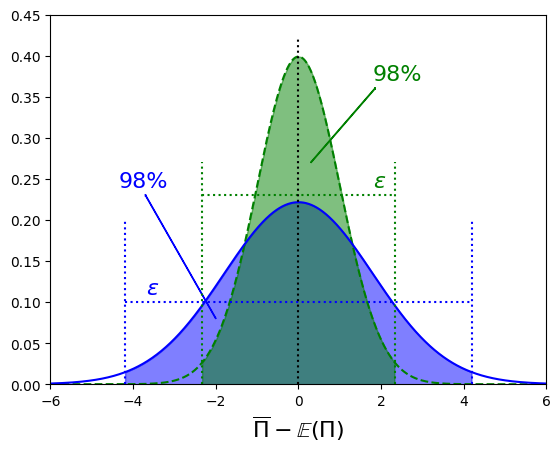
\includegraphics[width=0.9\linewidth]{confidence_interval}
\end{columns}
	\begin{tikzpicture}[remember picture,overlay]
	\node[xshift=5cm,yshift=-3.7cm] (image) at (current page.center) {
\includegraphics[width=20px]{python_logo}};
	\node[align = center, yshift=1.45cm, below=of image] {\tiny{\href{shorturl.at/NPQT1}{shorturl.at/NPQT1}}};
\end{tikzpicture}
\end{frame}

\begin{frame}{Monte Carlo Variance Reduction}
To reduce the confidence interval without running to much simulations, it can be used the control variate technique (i.e. reduce the sample variance, without increasing m).
\begin{enumerate}
\item Consider another payoff $\Pi_{an}$ which we can evaluate analytically, whose expectation is denoted by $\mathbb{E}[\Pi_{an}] = \pi_{an}$, and simulate it together with $\Pi$ under the same scenarios for $F$.
\item Define an unbiased estimator for $\mathbb{E}[\Pi]$ as the sample mean of the r.v. 
\begin{equation*}
\Pi_c(\gamma) = \Pi + \gamma(\Pi_{an} - \pi_{an})
\end{equation*}
Hence $\Pi_c(\gamma)$ has expectation $\mathbb{E}[\Pi]$ and variance
\begin{equation*}
Var(\Pi_c(\gamma)) = Var(\Pi) + \gamma^2 Var(\Pi_{an}) + 2\gamma Cov(\Pi, \Pi_{an})
\end{equation*}
This can be minimized by 
\begin{equation*}
\gamma^* = -\frac{Cov(\Pi, \Pi_{an})}{Var(\Pi_{an})} = -\frac{Corr(\Pi, \Pi_{an})}{Std(\Pi)Std(\Pi_{an})}
\end{equation*}
\end{enumerate}
\end{frame}

\begin{frame}{Monte Carlo Variance Reduction}
\begin{enumerate}
\setcounter{enumi}{2}
\item  The minimum variance of $\Pi_c$ is computed as
\begin{equation*}
Var(\Pi_c(\gamma^*)) = Var(\Pi) (1 - Corr(\Pi, \Pi_{an})^2)
\end{equation*}
that is smaller than the variance of $\Pi$; moreover, the larger the difference between the two variances the larger the correlation.
\item Moving to the standard deviation
\begin{equation*}
Std(\Pi_c(\gamma^*)) = Std(\Pi) \sqrt{(1 - Corr(\Pi, \Pi_{an})^2)}
\end{equation*}
the variance reduction will increase with the correlation between $\Pi$ and $\Pi_{an}$. 
\item Now if we consider the confidence interval for $\Pi_c$ 
\begin{equation*}
98\% C.L. =\left[\Pi_c(\gamma,m) - 2.33\cdot\frac{Std(\Pi_c)}{\sqrt{m}};\Pi_c(\gamma,m) + 2.33\cdot\frac{Std(\Pi_c)}{\sqrt{m}}\right] 
\end{equation*}
we get a narrower width by a factor of
\begin{equation*}
\sqrt{1 - Corr(\Pi, \Pi_{an}; m)^2}
\end{equation*}
\end{enumerate}
\end{frame}


\begin{frame}{Monte Carlo Variance Reduction}
\begin{itemize}
\item This technique is quite general and the choice of $\Pi_{an}$ is theoretically free.
\item In the case of the pricing of swaptions in the LFM, we select as $\Pi_{an}$ one of the simplest payoff with underlying rates $F_{\alpha+1},\ldots,F_\beta$, as may be a portfolio of FRA contracts at time $T_\alpha$ on each single time interval $(T_{i-1}, T_i]$.
\item Consider the payoff of such portfolio where the fair value at time 0 of $K$ is equal to $F_i(0)$ and rewrite it by a change of measure as follows:
%By recalling the price in (1.3) and reversing the two roles involved, we consider the $T^\alpha$-price 
%\begin{equation*}
%\sum_{i=\alpha+1}^\beta P(T_\alpha,T_i)\tau_i(F_i(T_\alpha)-K)
%\end{equation*}
%where the fair value at time 0 of $K$ is equal to $F_i(0)$. We take such contract as our $T^\alpha$-payoff and rewrite it by a change of measure as follows:
\begin{equation*}
\begin{aligned}
&\mathbb{E}^\mathcal{Q}\left[D(0,T_\alpha)\sum_{i=\alpha+1}^\beta P(T_\alpha,T_i)\tau_i(F_i(T_\alpha) - F_i(0))\right] = \\
&=\mathbb{E}^\mathcal{j}\left[\frac{P(0,T_i)}{P(T_\alpha,T_j)}\sum_{i=\alpha+1}^\beta P(T_\alpha,T_i)\tau_i(F_i(T_\alpha) - F_i(0))\right] = \\
& = P(0,T_j)\mathbb{E}^j\left[\frac{\sum_{i=\alpha+1}^\beta P(T_\alpha,T_i)\tau_i(F_i(T_\alpha) - F_i(0))}{P(T_\alpha,T_j)}\right]
\end{aligned}
\end{equation*}
\end{itemize}
\end{frame}

\begin{frame}{Monte Carlo Variance Reduction}
\begin{itemize}
\item Thus we can set
\begin{equation*}
\Pi_{an}(T_\alpha) = \frac{\sum_{i=\alpha+1}^\beta P(T_\alpha,T_i)\tau_i(F_i(T_\alpha) - F_i(0))}{P(T_\alpha,T_j)}
\end{equation*}
whose price at time 0 is $\pi_{an} = 0$.
\item  Indeed, the payoff $\Pi_{an}(\cdot)$ is a sum of traded assets divided by $P(\cdot, T_j)$, hence it is a martingale under the $T^j$-forward measure $\mathcal{Q}^j$, which implies that

\begin{equation*}
\mathbb{E}^j[\Pi_{an}(T_\alpha)] = \mathbb{E}^j[\Pi_{an}(0)] = \mathbb{E}^j[0] = 0
\end{equation*}
\end{itemize}
\end{frame}

\begin{frame}{Correlated Brownian Motions}
	\begin{itemize}
		\item In the LFM, we can assume that the Brownian motions driving the dynamics of forward rate are correlated
		\begin{equation}
			<dZ_t^{T_i}, dZ_t^{T_i}> = \rho_{ij}dt
		\end{equation}
		\item In models for short rate it is assumed full correlation $\rho_{ij}=1$, which is a tight constraint on the dynamics of the forward rates.
		\item In the LFM, we can allow decorrelation to better fit the derivatives at hand
		\begin{equation*}
			dF_k(t) = \sigma_kF_k\sum_{j=\alpha+1}^k\frac{\boxed{\rho_{kj}}\tau_j\sigma_jF_j}{1+\tau_jF_j}dt+\sigma_kF_k dZ^\alpha_k
		\end{equation*}
	\end{itemize}
\end{frame}

\begin{frame}{Correlation}
\begin{itemize}
\item Correlation is a linear measure of dependency between random variables. Given two random variables $X$ and $Y$, their correlation is given by

\begin{equation*}
	\rho_{X,Y} = \frac{\mathbb{E}((X-\mathbb{E}(X))(Y-\mathbb{E}(Y))}{\sigma_X \sigma_Y}
\end{equation*}

\item Correlation can be estimated from historical market data: forward rates are retrieved from daily swap curves.
\item To estimate instantaneous correlation that is consistent with the LIBOR market model, log-returns of the forward rates are calculated:

\begin{equation*}
	f_i(t_j) := \log\left(\frac{F(t_j, T_{i-1}, T_i)}{F(t_{j-1}, T_{i-1}, T_i)}\right), \quad j=2,\ldots,n
\end{equation*}

where $n$ is the number of daily forward rates. %Therefore, each series of log-normal forward rate returns corresponds to a LIBOR rate of the LIBOR market model as given by equation (2.11). 
\item  An $M \times M$ correlation matrix was then calculated for each yearly data set.
\end{itemize}
\end{frame}

\begin{frame}{Correlation Parametrization}
\begin{itemize}
\item Many parametrization functions have been introduced to express a given correlation matrix of forward rates in a functional form. 
\item This has several advantages: it is computationally convenient to work with an analytical formula. Noise (e.g. non-synchronous data or illiquidity) is removed by focussing on general properties of correlation. Furthermore, the correlation matrix rank can be controlled through the functional form.
\item One property that is always implicitly present is time-homogeneity: correlation of forward rates does not depend on calendar time $t$, but only on the rates’ time to maturity $T_i-t$.
%An important aspect of these parameterizations is the number of parameters used to fit the market data. Most parameterizations advocate the use of few parameters that emphasize general properties of market correlation and prevent overfitting.
\item  General requirements on an $M \times M$ correlation matrix $\rho$ are:
\begin{enumerate}
	\item $\rho$ must be real and symmetric;
	\item $\rho_{i,i}=1$ for $i = 1,\ldots, M$;
	\item $\rho$ must be positive semidefinite such that can be decomposed into $\rho = BB^T$.
\end{enumerate}
\item Usually parameterizations are determined by minimizing the mean square error between historical market correlation and parameterized functional form.
\end{itemize}
\end{frame}

\begin{frame}{Instantaneous and Terminal Correlation}
\begin{itemize}
\item For calibrating a LIBOR market model, instantaneous
correlation is modeled. However, for pricing correlation-sensitive products, terminal correlation is used.
\item It is important to understand how this instantaneous correlation in the forward-rate dynamics translates into a terminal correlation of simple rates.
%\item Define an $n$-dimensional LFM with $m$ factors:
%\begin{equation*}
%	\frac{df_i}{f_i} = \mu_i dt + \sigma_i \sum_{k=1}^m b_{ik}dZ_k
%\end{equation*}
%with $b_k=\frac{\sigma_{ik}}{\sqrt{\sum_{k=1}^m\sigma_{ik}^2}}$
	
\begin{block}{Definition}
The \textcolor{red}{instantaneous correlation} is a quantity summarizing the degree of “dependence” between changes of different forward rates.
\begin{equation*}
\rho_{ij} = \frac{dF_i(t) dF_j(t)}{Std(dF_i(t)) Std(dF_j(t))}
\end{equation*}
%where $Std$ denotes the standard deviation conditional on the information available at time $t$ at which the change occurs. 
%The instantaneous correlation of the LIBOR rates $L(t, T_{i-1}, T_i)$ and $L(t, T_{j-1}, T_j)$ is given by the correlation of the increments of the Brownian motions:
%\begin{equation*}
%\rho_{i,j}(t) = \sum_{k=1}^m b_{i,k}b_{j,k}, \quad i,j=1,\ldots,n
%\end{equation*}
%From this formula it is clear that indeed the instantaneous correlation ρ is related to changes dF in for- ward rates. Instead, 
The \textcolor{red}{terminal correlation} is a quantity summarizing the degree of “dependence” between two different forward rates at a given \emph{terminal} time-instant. Typically, the $T_1$ terminal correlation between $F_i$ and $F_j$ is the correlation between $F_i(T_1)$ and $F_j(T_1)$.
\end{block}
	
%\begin{block}{Definition}
%The terminal correlation of the LIBOR rates$L(t, T_{i-1}, T_i)$ and $L(t, T_{j-1}, T_j)$ is given by
%\begin{equation*}
%\tilde{\rho}_{i,j}(t) = %\frac{\int_o^t\sigma_i(u)\sigma_j(u)\rho_{i,j}(u)du}{\sqrt{\int_0^t\sigma_i(u)^2du\int_o^t\sigma_j(u)^2du}}
%\end{equation*}
%\end{block}
\end{itemize}
\end{frame}

\begin{frame}{Decorrelation}
\begin{itemize}
	\item Is this terminal correlation completely determined by the instantaneous correlations $\rho_{ij}$ between $Z_i$ and $Z_j$ ?
	\item If \textcolor{red}{instantaneous volatilities} are not constant, they have a significant impact on terminal correlation and can produce terminal decorrelation, even in the case of perfect instantaneous correlation.
	\item Prices of correlation-sensitive products depend on terminal correlation, and thus instantaneous correlation and instantaneous volatility. 
	\item It is important to note that there is no instrument that is sensitive solely to instantaneous correlation. Therefore, estimating correlation from a product that is sensitive to multiple factors is not straight-forward and can lead to ambiguous results.
\end{itemize}
\end{frame}

\begin{frame}{An Example}
As an example, considers swaption prices that terminal correlation can be inferred from.
In the case of constant volatilities, terminal correlation is just the average correlation over the period. To see this, consider the Rebonato analytical formula for $\rho$
\begin{equation*}
\tilde{\rho}_{ij}(t)=\frac{\int_0^t\sigma_i(u)\sigma_j(u)\rho_{ij}(u)du}{\sqrt{\int_0^t\sigma_i(u)^2 du\int_0^t\sigma_j(u)^2 du}}	
\end{equation*}
Since the instantaneous volatilities are constant, they can be factored out from the integrals
\begin{equation*}
\tilde{\rho}_{ij}(t)=\frac{\cancel{\sigma_i}\cancel{\sigma_j}\int_0^t\rho_{ij}(u)du}{\sqrt{\cancel{\sigma_i^2}\cancel{\sigma_j^2} t^2}}= \frac{\int_0^t\rho_{ij}(u)du}{t}		
\end{equation*}
\end{frame}

\end{document}
